% =====================================================================
%  Unit 5 -- Deployment of models
%  (this file is assembled from src/ch05/*.tex by build_chapter.py)
% =====================================================================
\chapter{Deployment of Models}\label{ch:deployment}

On the morning of 1 August 2012, Knight Capital, one of the largest traders of American equities, started using new
software on the servers that sent its orders to the stock market. A technician had not copied the new code to one of
the eight servers, where an obsolete function, reactivated by a flag that the new code reused, began to send orders
that nobody had intended. In 45 minutes the firm lost more than 460 million dollars; it had to be rescued by investors
and was taken over the following year \citep{sec2013knight}. Knight's software was not a machine learning model, but
its failure is the nightmare of every deployment: a manual step, no automated check that every server ran the same
version, and no quick way of stopping. Deploying models adds risks of its own to these.

A prediction model creates value only when its users can reach its outputs reliably. Deployment is the step that puts a model in front
of its users, and it is where many data science projects fail: surveys of practitioners describe
models that worked in the laboratory and never reached production, or reached it and broke
\citep{paleyes2022challenges}. This unit covers the two halves of the problem. The first is
choosing \emph{how} a model will serve its predictions: on a server that answers requests one by
one or in batches, on the user's own device, and, for training, federated learning, which learns
from data that stay on the devices and can produce a shared model or personalised ones. The second is building the \emph{infrastructure} that makes deployment
reliable and repeatable: version control for code and data, experiment tracking, automated tests,
packaging, and pipelines that retrain and redeploy models automatically, a set of practices known
as ModelOps or MLOps \citep{kreuzberger2023mlops}. We follow the approach of
\citet{ameisen2020building} for the first half and of \citet{dubovikov2019managing} for the
second.

\begin{objectives}
After studying this unit you should be able to:
\begin{itemize}
  \item choose a deployment option (server-side streaming or batch, client-side on device or in
        the browser, federated learning) from the latency, hardware, network, privacy, cost and
        complexity requirements of an application;
  \item build a prediction API, and measure its latency and throughput;
  \item make a model small enough for a device, and explain how federated learning trains
        personalised models without collecting the data;
  \item exchange models between platforms with standard formats such as PMML and ONNX, and
        build and test a small web application for a model;
  \item explain ModelOps and its relation to DevOps, and set up version control for code and data,
        reproducible environments and experiment tracking;
  \item write automated tests for data science code, package it, and design a continuous training
        pipeline with data tests and quality gates;
  \item assemble a technology stack for a data science team.
  \item deploy applications built on large language models: choose where the model runs, treat prompts
        as code, build and evaluate retrieval-augmented generation, and add guardrails;
\end{itemize}
\end{objectives}

% =====================================================================
\section{Choosing a deployment option}\label{sec:deployoptions}

Different deployment approaches suit different requirements. Before choosing one we must consider
the \emph{latency} the application can tolerate, the \emph{hardware} and \emph{network} available
at prediction time, the \emph{privacy} of the data, the \emph{cost} of running the system and the
\emph{complexity} we can afford to maintain. \Cref{tab:deploy} summarises how the options of this
section compare.

\begin{table}[htbp]
\centering\small
\caption{Deployment options and their trade-offs.}\label{tab:deploy}
\begin{tabularx}{\textwidth}{@{}>{\raggedright\arraybackslash}p{2.5cm}>{\raggedright\arraybackslash}X>{\raggedright\arraybackslash}X@{}}
\toprule
Option & When it fits & Main costs and risks\\
\midrule
Server, streaming (API) & the data needed are known only at request time and the prediction is
needed immediately & servers that scale with the number of users; a central point of failure\\
Server, batch & the features are available before the prediction is needed & predictions can be
stale; storage of precomputed results\\
Client, on device & low latency without network, offline use, sensitive data & small models,
possible loss of accuracy, one optimisation per type of device\\
Client, browser & interactive applications without installation & the model is downloaded by every
visitor\\
Federated learning (training) & the training data must stay on the devices; it learns a shared model, which
can then be personalised &
much greater complexity: training, aggregation and privacy on many devices\\
\bottomrule
\end{tabularx}
\end{table}

\subsection{Server-side deployment}

Server-side deployment sets up a web server that accepts requests from clients, runs them through an
inference pipeline, and returns the results. There are two common workloads: \emph{streaming}, in
which each request is answered as it arrives, and \emph{batch}, in which predictions are computed in
advance for many examples (\cref{fig:serverflows}).

\begin{figure}[htbp]
\centering
\begin{tikzpicture}[font=\scriptsize\sffamily,
  st/.style={draw=edmnavy,fill=edmnavy!6,rounded corners=2pt,minimum height=8mm,minimum width=15.5mm,align=center},
  ds/.style={cylinder,shape border rotate=90,draw=edmnavy,fill=edmbronze!25,aspect=0.25,minimum width=11mm,minimum height=8mm,align=center},
  arr/.style={-{Stealth[length=1.6mm]},edmnavy},
  lab/.style={font=\scriptsize\sffamily\bfseries,text=edmnavy,anchor=east,align=right}]
  \node[lab] at (-0.95,0) {streaming\\(per request)};
  \node[st] (r) at (0,0) {request};
  \node[st] (v) at (1.95,0) {validate};
  \node[st] (g) at (3.9,0) {gather\\more data};
  \node[st] (p) at (5.85,0) {pre-\\process};
  \node[st] (m) at (7.8,0) {run the\\model};
  \node[st] (o) at (9.75,0) {post-\\process};
  \node[st] (s) at (11.7,0) {send the\\result};
  \node[ds] (d1) at (3.9,-1.35) {store};
  \foreach \a/\b in {r/v,v/g,g/p,p/m,m/o,o/s} \draw[arr] (\a) -- (\b);
  \draw[arr,{Stealth[length=1.6mm]}-{Stealth[length=1.6mm]}] (g) -- (d1);
  \begin{scope}[yshift=-3.1cm]
  \node[lab] at (-0.95,0) {batch\\(scheduled)};
  \node[st] (bg) at (0.98,0) {gather all\\the data};
  \node[st] (bp) at (3.9,0) {pre-\\process all};
  \node[st] (bm) at (6.83,0) {run the\\model};
  \node[st] (bo) at (9.75,0) {post-\\process};
  \node[ds] (bs) at (11.7,0) {stored\\results};
  \foreach \a/\b in {bg/bp,bp/bm,bm/bo,bo/bs} \draw[arr] (\a) -- (\b);
  \end{scope}
  \begin{scope}[yshift=-4.75cm]
  \node[lab] at (-0.95,0) {batch\\(per request)};
  \node[st] (qr) at (0,0) {request};
  \node[st,minimum width=26mm] (ql) at (5.85,0) {look up the\\stored prediction};
  \node[st] (qs) at (9.75,0) {send the\\result};
  \draw[arr] (qr) -- (ql);
  \draw[arr] (ql) -- (qs);
  \draw[arr,dashed] (bs.south) -- ++(0,-0.25) -| (ql.north);
  \end{scope}
\end{tikzpicture}
\caption{Server-side inference. A streaming request goes through the whole pipeline; a batch job
computes the predictions in advance, and requests only look them up.}
\label{fig:serverflows}
\end{figure}

\paragraph{Streaming applications} The streaming approach treats the model as an \emph{endpoint}
to which users send requests; the users can be the end users of an application or an internal
service that relies on the predictions (for instance, a service that adjusts the number of servers
to the predicted traffic of a website). The code path of a request goes through six steps:
\emph{validate} the request (its values and the caller's permissions), \emph{gather} any additional
data the model needs, \emph{preprocess} the data, \emph{run} the model, \emph{postprocess} the results
(check that they are within bounds, make them understandable) and \emph{return} them. A streaming
approach is needed when the information the model requires is available only at prediction time and
the prediction is required immediately: a ride-hailing application that quotes the price of a trip
needs the user's location and the current availability of drivers, which exist only when the user
asks.

\Cref{lst:api} implements such an endpoint with Flask, the framework used by the ML Editor example of
\citet{ameisen2020building}. It follows the six steps, and its response codes tell the client what
went wrong: a valid request gets a probability, a decision and the version of the model (always
worth returning, for debugging and monitoring); a non-numeric value or a value out of range gets a
400 error, an unknown customer a 404, and a wrong key a 401. With Flask's test client, which skips
the network, a request takes less than a millisecond. In production the application runs behind a
WSGI server with several workers, and usually behind a load balancer.

\begin{pylisting}[label={lst:api}]{A prediction API with Flask, following the six steps of a request}
import time
import numpy as np
from flask import Flask, jsonify, request
from sklearn.datasets import make_classification
from sklearn.ensemble import GradientBoostingClassifier

# Offline: train the model and fill a feature store with data known before any request
X, y = make_classification(n_samples=3000, n_features=4, n_informative=4, n_redundant=0,
                           random_state=0)
model = GradientBoostingClassifier(random_state=0).fit(X, y)
store = {f"c{i:04d}": X[i, 2:] for i in range(len(X))}       # history of each customer
VERSION = "1.3.0"
app = Flask(__name__)

@app.post("/predict")
def predict():
    body = request.get_json(silent=True)
    if not isinstance(body, dict):                          # 1. validate: structure,
        return jsonify(error="a JSON object is required"), 400
    if body.get("api_key") != "secret":                     #    permissions
        return jsonify(error="not authorised"), 401
    if not isinstance(body.get("customer"), str):
        return jsonify(error="customer must be a string"), 400
    try:                                                    #    and values
        if any(isinstance(body.get(k), bool) for k in ("f1", "f2")):
            raise TypeError
        x = np.array([float(body["f1"]), float(body["f2"])])
    except (KeyError, TypeError, ValueError, OverflowError):
        return jsonify(error="f1 and f2 must be numbers"), 400
    if not np.isfinite(x).all() or np.any(np.abs(x) > 10):
        return jsonify(error="f1 and f2 must be finite and in [-10, 10]"), 400
    history = store.get(body["customer"])                         # 2. gather more data
    if history is None:
        return jsonify(error="unknown customer"), 404
    features = np.r_[x, history].reshape(1, -1)                   # 3. preprocess
    p = float(model.predict_proba(features)[0, 1])                # 4. run the model
    return jsonify(probability=p, version=VERSION,                # 5. postprocess
                   decision="accept" if p >= 0.5 else "reject")   # 6. return

client = app.test_client()                 # in production: an HTTP server and clients
good = {"api_key": "secret", "customer": "c0007", "f1": 0.5, "f2": -1.2}
requests = [good, {**good, "f1": "high"}, {**good, "f1": "NaN"}, [1, 2],
            {**good, "customer": "c9999"}, {**good, "f2": 45},
            {**good, "api_key": "guess"}]
for body in requests:
    r = client.post("/predict", json=body)
    print(r.status_code, r.get_json())
start = time.perf_counter()
for _ in range(200):
    client.post("/predict", json=good)
print(f"mean latency: {(time.perf_counter() - start) / 200 * 1000:.1f} ms per request")
\end{pylisting}
\begin{pyoutput}
200 {'decision': 'reject', 'probability': 0.2614178950022486, 'version': '1.3.0'}
400 {'error': 'f1 and f2 must be numbers'}
400 {'error': 'f1 and f2 must be finite and in [-10, 10]'}
400 {'error': 'a JSON object is required'}
404 {'error': 'unknown customer'}
400 {'error': 'f1 and f2 must be finite and in [-10, 10]'}
401 {'error': 'not authorised'}
mean latency: 0.5 ms per request
\end{pyoutput}

The validation step rejects malformed requests (a list instead of an object, a text or an infinite value
where a number is expected) with an error 400 before the model is called, and the probability is
returned without rounding, so that a client can reproduce the decision from it.

The endpoint approach is quick to implement, but the infrastructure has to grow with the number of
users: if the traffic exceeds the capacity of the servers, requests are delayed or fail. A useful tool
for sizing it is \emph{Little's law} \citep{little1961proof}: in a stable system, the mean number of
requests being served, $L$, equals the arrival rate $\lambda$ times the mean time each request spends
in the system, $W$,
\begin{equation}\label{eq:little}
  L=\lambda\,W .
\end{equation}
At 200 requests per second and 50 milliseconds per request, 10 requests are in progress on average,
so a server that can handle four at a time is not enough. Means are not the whole story: users
experience the \emph{tail} of the latency distribution, and in systems that call many services a few
slow responses dominate the user experience, which is why latency objectives are stated as high
percentiles such as p95 or p99 \citep{dean2013tail}.

\paragraph{Batch predictions} A batch job runs a model on many examples at a scheduled time and stores
the predictions, so that they can be looked up when they are needed. It is appropriate when the
features are available before the prediction is required. A model that helps salespeople decide which
prospects to contact can be trained on historical conversations and market trends, all known in
advance, and score every prospect overnight; an application that ranks the notifications a user
should read in the morning can process all unread messages in one batch before the user wakes up. A
batch approach needs as many inferences as a streaming one, but it is more resource efficient:
because the number of predictions is known at the start, resources are easy to allocate and
parallelise, and many examples can be processed per call. And at request time, looking up a stored
prediction is faster than computing it.

\begin{pylisting}[label={lst:latency}]{Latency of single requests and throughput of batches}
import time
import numpy as np
from sklearn.datasets import make_classification
from sklearn.ensemble import RandomForestClassifier

X, y = make_classification(n_samples=20000, n_features=20, random_state=0)
model = RandomForestClassifier(200, n_jobs=1, random_state=0).fit(X[:5000], y[:5000])
pool = X[5000:]

latency = []                                       # streaming: one request per call
for i in range(500):
    start = time.perf_counter()
    model.predict_proba(pool[i:i + 1])
    latency.append((time.perf_counter() - start) * 1000)
p50, p95, p99 = np.percentile(latency, [50, 95, 99])
print(f"single requests: p50 {p50:.1f} ms, p95 {p95:.1f} ms, p99 {p99:.1f} ms")

throughput = {}                                    # batch: many examples per call
for size in (1, 10, 100, 1000, 10000):
    reps = max(3, 300 // size)
    start = time.perf_counter()
    for _ in range(reps):
        model.predict_proba(pool[:size])
    throughput[size] = size * reps / (time.perf_counter() - start)
    print(f"batches of {size:5d}: {throughput[size]:9,.0f} predictions per second")
\end{pylisting}
\begin{pyoutput}
single requests: p50 9.9 ms, p95 10.5 ms, p99 11.2 ms
batches of     1:       101 predictions per second
batches of    10:       969 predictions per second
batches of   100:     7,305 predictions per second
batches of  1000:    31,478 predictions per second
batches of 10000:    57,923 predictions per second
\end{pyoutput}

\Cref{lst:latency} and \cref{fig:serving} quantify the difference for a random forest of 200 trees. A
single request takes about 10 milliseconds (p50 9.9, p95 10.5 and p99 11.2), so one process answers
about 100 requests per second. Called with batches of 10,000 examples, the same model produces about
58,000 predictions per second, almost 600 times more, because the fixed cost of each call (checking
the input, dispatching to the 200 trees) is shared by many examples.

\begin{figure}[htbp]
\centering
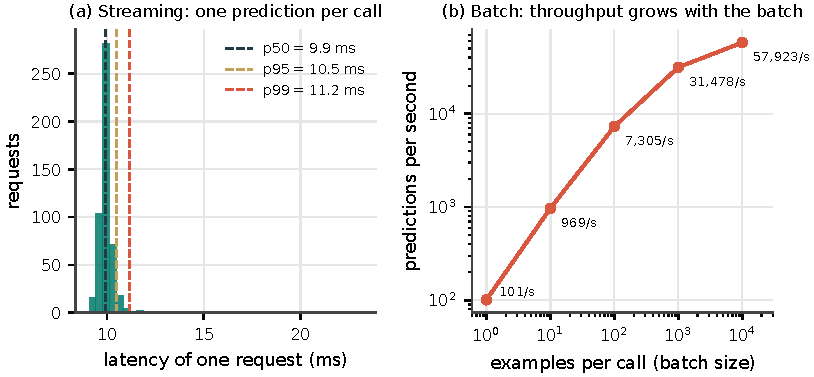
\includegraphics[width=\textwidth]{ch05/serving_latency}
\caption{(a) Latency of 500 single-example requests to a random forest, with its percentiles.
(b) Throughput as a function of the number of examples per call (both axes logarithmic).}
\label{fig:serving}
\end{figure}

A \emph{hybrid} approach precomputes as many cases as possible and, at inference time, either retrieves
the stored result or computes it on the spot if it is missing or outdated. It combines the speed of
batch with the freshness of streaming, at the price of a significantly more complex system. All
server-side approaches share two drawbacks: hosting servers to run inference for every customer can
quickly become expensive if the product becomes popular, and the servers are a central point of
failure for the application.

\subsection{Client-side deployment}

The goal of client-side deployment is to run all the computation on the client, eliminating the need
for a server to run models. Models are usually trained in the same way, on a powerful server, and are
then sent to the device, through an application or a web browser, which runs the inference. This
reduces the infrastructure needed to serve every user, reduces the amount of data transferred between
device and server, and keeps sensitive data on the device: sending user data to the cloud, and storing
it even temporarily, increases the chances that an attacker gets access to it. The main limitation is
the complexity of the models that can be used.

\paragraph{On the device} A model that runs on a laptop or a phone should be as small as possible, to
run quickly and without draining the battery. There are several ways of shrinking it: using a simpler
model, reducing the number of parameters or the \emph{precision} of the computations (quantisation,
\citealp{jacob2018quantization}; pruning, \citealp{han2016deep}), reducing the number of features, or
distilling a large model into a small one (\cref{sec:drawbacks}). Specialised runtimes, such as
TensorFlow Lite or ONNX Runtime (\cref{sec:exchange}), execute the result efficiently. Most models
lose a little performance when they are ported to a device; if the product cannot tolerate that
degradation, the model must stay on a server. Latency matters too: if running the model on the device
takes longer than sending the data to a server and waiting for the answer, the server may be the better
option. For many applications, though, the value of a local model that works without connection
outweighs a small loss of accuracy: predictive keyboards, applications that identify plants from a
photo taken on a hike, or translators.

\begin{pylisting}[label={lst:ondevice}]{Shrinking a model for a device: fewer trees, lower precision, fewer features}
import pickle
import numpy as np
from sklearn.datasets import load_digits
from sklearn.ensemble import RandomForestClassifier
from sklearn.linear_model import LogisticRegression
from sklearn.model_selection import train_test_split
from sklearn.neural_network import MLPClassifier
from sklearn.tree import DecisionTreeClassifier

X, y = load_digits(return_X_y=True)
X = X / 16.0
X_tr, X_te, y_tr, y_te = train_test_split(X, y, test_size=0.4, random_state=0, stratify=y)
kb = lambda obj: len(pickle.dumps(obj)) / 1024             # what we ship to the device
results = []
for n in (300, 30):
    rf = RandomForestClassifier(n, random_state=0).fit(X_tr, y_tr)
    results.append((f"random forest, {n} trees", kb(rf), rf.score(X_te, y_te)))
tree = DecisionTreeClassifier(max_depth=10, random_state=0).fit(X_tr, y_tr)
results.append(("decision tree, depth 10", kb(tree), tree.score(X_te, y_te)))

mlp = MLPClassifier((64,), max_iter=1000, random_state=0).fit(X_tr, y_tr)
def mlp_accuracy(W, b):                              # inference with given weights
    h = np.maximum(X_te @ W[0].astype(float) + b[0], 0)
    return np.mean(np.argmax(h @ W[1].astype(float) + b[1], axis=1) == y_te)
b = [v.astype(np.float32) for v in mlp.intercepts_]
for dtype in (np.float32, np.float16):               # lower precision
    W = [w.astype(dtype) for w in mlp.coefs_]
    results.append((f"neural network, {np.dtype(dtype).name}", kb((W, b)),
                    mlp_accuracy(W, b)))
scales = [np.abs(w).max() / 127 for w in mlp.coefs_]  # int8: one scale per layer
Wq = [np.round(w / s).astype(np.int8) for w, s in zip(mlp.coefs_, scales)]
results.append(("neural network, int8", kb((Wq, scales, b)),
                mlp_accuracy([q * s for q, s in zip(Wq, scales)], b)))

top = np.argsort(-rf.feature_importances_)[:16]        # fewer features: 16 pixels
lr = LogisticRegression(max_iter=2000).fit(X_tr[:, top], y_tr)
W16, b16 = lr.coef_.astype(np.float16), lr.intercept_.astype(np.float16)
scores = X_te[:, top] @ W16.astype(float).T + b16.astype(float)   # the stored values
acc16 = np.mean(lr.classes_[scores.argmax(axis=1)] == y_te)
results.append(("logistic, 16 pixels, float16", kb((W16, b16, top)), acc16))
for name, size, acc in sorted(results, key=lambda r: -r[1]):
    print(f"{name:30s} {size:8.1f} KiB   accuracy {acc:.3f}")
\end{pylisting}
\begin{pyoutput}
random forest, 300 trees        11897.6 KiB   accuracy 0.971
random forest, 30 trees          1203.2 KiB   accuracy 0.967
decision tree, depth 10            26.9 KiB   accuracy 0.839
neural network, float32            19.0 KiB   accuracy 0.974
neural network, float16             9.8 KiB   accuracy 0.974
neural network, int8                5.3 KiB   accuracy 0.975
logistic, 16 pixels, float16        0.7 KiB   accuracy 0.928
\end{pyoutput}

\Cref{lst:ondevice} and \cref{fig:ondevice} compare models for recognising handwritten digits by the
number of kilobytes that would have to be shipped to the device. A random forest of 300 trees reaches
an accuracy of 0.971 but its serialised artefact occupies 11.6~MiB (11,898~KiB), and ten times fewer trees still
need 1.2~MiB. A small neural
network is both smaller and as accurate: 19~KiB in 32-bit floating point, 9.8~KiB in 16-bit, and 5.3~KiB
when its weights are quantised to 8-bit integers with one scale per layer, with no loss of accuracy
(0.975). A logistic regression that uses only 16 of the 64 pixels fits in 0.7~KiB, at the price of four
points of accuracy. The neural network in \texttt{int8} is more than 2000 times smaller than the large
forest, with the same accuracy. These sizes are those of the serialised parameters; the example quantises the stored weights and
checks the predictions after converting them back to floating point, so it does not measure a complete
mobile package, the peak memory, or the speed of integer arithmetic, which must be measured on the
target device.

\begin{figure}[htbp]
\centering
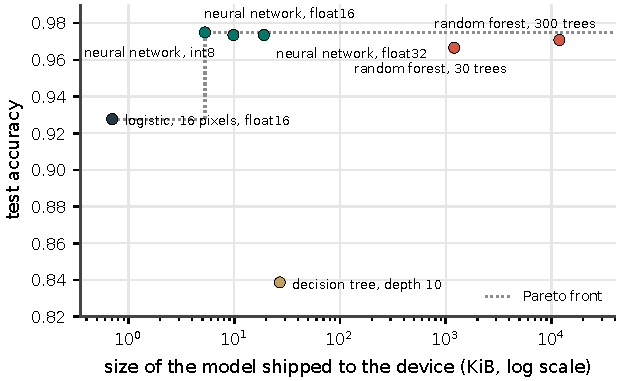
\includegraphics[width=0.78\textwidth]{ch05/on_device}
\caption{Accuracy and size of several models for digit recognition. The dotted line is the Pareto
front: no model is both smaller and more accurate than the models on it.}
\label{fig:ondevice}
\end{figure}

\paragraph{In the browser} Browsers are optimised for fast graphical computation, and libraries such
as TensorFlow.js \citep{smilkov2019tensorflowjs} can train and run most differentiable models in
JavaScript. Users interact with the model without installing anything, and the computation happens on
their devices. The drawback is bandwidth: the model must be downloaded by each visitor (caching helps
when they come back), which again favours small models.

\subsection{Federated learning}

So far we have deployed a single model, trained in advance, for all users. What if each user needed a
different model, as in content recommendation or healthcare? One solution is to give a shared model
user-specific features. Another is \emph{federated learning} \citep{mcmahan2017communication,kairouz2021advances}:
every user has a model with the same architecture but different parameter values; each model learns
from its user's data, and only sends model updates to a server, which aggregates them to improve a
global model and sends it back to the clients (\cref{fig:fedround}). Each user receives a model that
benefits from what all the others have learned, and the data never leave the devices.

\begin{figure}[htbp]
\centering
\begin{tikzpicture}[font=\scriptsize\sffamily,
  srv/.style={draw=edmnavy,fill=edmnavy!8,rounded corners=3pt,minimum width=40mm,minimum height=10mm,align=center},
  dev/.style={draw=edmteal,fill=edmteal!10,rounded corners=4pt,minimum width=23mm,minimum height=12mm,align=center},
  down/.style={-{Stealth[length=1.8mm]},edmnavy,thick},
  up/.style={-{Stealth[length=1.8mm]},edmcoral,thick}]
  \node[srv] (s) at (0,0) {server: $w\leftarrow\sum_k\frac{n_k}{n}\,w_k$\\(4) aggregate the updates};
  \foreach \i/\x in {1/-4.2,2/0,3/4.2} {
    \node[dev] (d\i) at (\x,-2.9) {client \i\\(2) train on its own\\private data};
    \draw[down] ([xshift=-3mm]s.south) ++(0,0) -- ([xshift=-3mm]d\i.north);
    \draw[up] ([xshift=3mm]d\i.north) -- ([xshift=3mm]s.south);
  }
  \node[text=edmnavy,align=right,anchor=east] at (-4.4,-1.25) {(1) the server sends\\the global model $w$};
  \node[text=edmcoral,align=left,anchor=west] at (4.4,-1.25) {(3) each client sends\\back its model $w_k$};
\end{tikzpicture}
\caption{A round of federated averaging: the global model goes down, each client trains it on its
private data and sends it back, and the server averages the local models, weighting each by the
number of examples $n_k$ of its client.}
\label{fig:fedround}
\end{figure}

In \emph{federated averaging} (FedAvg, \citealp{mcmahan2017communication}), the most common algorithm,
each round sends the current global model $w$ to the clients; client $k$ runs a few epochs of
stochastic gradient descent on its $n_k$ examples, obtaining $w_k$; and the server replaces $w$ by the
weighted average $\sum_k(n_k/n)\,w_k$, with $n=\sum_kn_k$. Google's mobile keyboard used federated
learning to improve next-word prediction from the typing of its users without collecting what they
typed \citep{hard2018federated}.

\begin{pylisting}[label={lst:fedavg}]{Federated averaging from scratch, with non-IID clients and personalisation}
import numpy as np
from sklearn.datasets import load_digits
from sklearn.model_selection import train_test_split

rng = np.random.default_rng(0)
X, y = load_digits(return_X_y=True)
X = X / 16.0
X_pool, X_test, y_pool, y_test = train_test_split(X, y, test_size=0.3, random_state=0,
                                                  stratify=y)
K = 10                                             # clients, e.g. phones of 10 users
favourite = (y_pool + rng.integers(0, 2, len(y_pool))) % K   # each digit: 2 clients
to_favourite = rng.random(len(y_pool)) < 0.8                 # 80% go to a favourite
owner = np.where(to_favourite, favourite, rng.integers(0, K, len(y_pool)))
clients = []                                       # non-IID data: (train, own test)
for k in range(K):
    idx = rng.permutation(np.flatnonzero(owner == k))
    cut = int(0.7 * len(idx))
    clients.append((X_pool[idx[:cut]], y_pool[idx[:cut]],
                    X_pool[idx[cut:]], y_pool[idx[cut:]]))

def sgd(W, X, y, epochs, lr=0.5, batch=16):
    """Mini-batch SGD for softmax regression; the last row of W is the bias."""
    W, Xb, Y = W.copy(), np.c_[X, np.ones(len(X))], np.eye(10)[y]
    for _ in range(epochs):
        perm = rng.permutation(len(X))
        for s in range(0, len(X), batch):
            j = perm[s:s + batch]
            Z = Xb[j] @ W
            P = np.exp(Z - Z.max(axis=1, keepdims=True))
            W -= lr * Xb[j].T @ (P / P.sum(axis=1, keepdims=True) - Y[j]) / len(j)
    return W

acc = lambda W, X, y: np.mean(np.argmax(np.c_[X, np.ones(len(X))] @ W, axis=1) == y)
own = lambda models: np.mean([acc(W, c[2], c[3]) for W, c in zip(models, clients)])
W0, n = np.zeros((65, 10)), np.array([len(c[1]) for c in clients])
W, history = W0, []
for rnd in range(30):                              # federated averaging (FedAvg)
    local = [sgd(W, c[0], c[1], epochs=2) for c in clients]      # on the devices
    W = sum(nk * Wk for nk, Wk in zip(n, local)) / n.sum()       # on the server
    history.append(acc(W, X_test, y_test))
central = sgd(W0, np.vstack([c[0] for c in clients]),
              np.concatenate([c[1] for c in clients]), epochs=60)
alone = [sgd(W0, c[0], c[1], epochs=60) for c in clients]
tuned = [sgd(W, c[0], c[1], epochs=2) for c in clients]          # personalisation
print("model                        all digits   each user's own data")
results = {}
for name, models in [("centralised (data pooled)", [central] * K),
                     ("local models only", alone), ("federated averaging", [W] * K),
                     ("federated + fine-tuning", tuned)]:
    everyone = np.mean([acc(m, X_test, y_test) for m in models])
    results[name] = (everyone, own(models))
    print(f"{name:28s}    {everyone:.3f}          {own(models):.3f}")
print(f"each round: {K} clients x {W.size} parameters each way; no data leaves a device")
\end{pylisting}
\begin{pyoutput}
model                        all digits   each user's own data
centralised (data pooled)       0.965          0.969
local models only               0.562          0.874
federated averaging             0.952          0.935
federated + fine-tuning         0.854          0.969
each round: 10 clients x 650 parameters each way; no data leaves a device
\end{pyoutput}

\Cref{lst:fedavg} simulates ten users whose data are \emph{non-IID}, as they are in practice: each user
writes mostly two of the ten digits. A softmax regression is trained in four ways (\cref{fig:federated}).
Pooling all the data on a server, which federated learning forbids, gives an accuracy of 0.965 on all
the digits. A model trained only on each user's data is good at that user's digits (0.874) but poor at
the others (0.562). Federated averaging reaches 0.952 on all the digits after 30 rounds, without any
example leaving its device; and fine-tuning the federated model for two epochs on each device gives
every user a personalised model, and the mean accuracy across clients on their own test data (0.969) matches
that of the centralised model. The mean hides differences: in this run some clients gain and others lose
accuracy with fine-tuning, so the distribution across clients should be reported too. Note that federated
learning concerns how a model is \emph{trained}; the resulting model can then serve predictions on the devices
or on a server.
Personalisation has a cost, though: the fine-tuned models are worse on the digits their users rarely
write (0.854), a trade-off that depends on whether the user's future data will look like their past
data.

\begin{figure}[htbp]
\centering
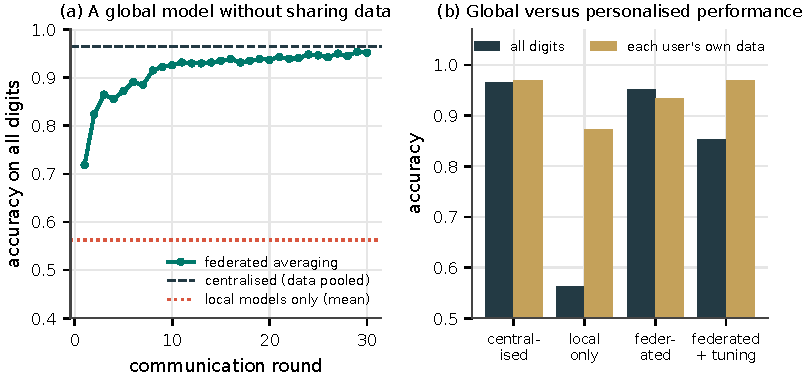
\includegraphics[width=\textwidth]{ch05/federated}
\caption{Federated learning on non-IID digits. (a) Accuracy of the federated model after each
communication round. (b) Accuracy on all the digits and on each user's own data for the four
strategies.}
\label{fig:federated}
\end{figure}

Federated learning is an exciting direction, but it adds a layer of complexity
\citep{li2020federated}: making sure that each individual model performs well, coping with clients
that are slow, offline or malicious, and limiting communication. And keeping the data on the device
is not enough to guarantee privacy, since model updates can leak information about the training
examples \citep{zhu2019deep}; secure aggregation, which lets the server see only the sum of the updates
\citep{bonawitz2017practical}, and differential privacy, which adds calibrated noise
\citep{abadi2016deep}, are used to close that gap.

% =====================================================================
\section{Exchanging and packaging models}\label{sec:exchange}

The environment where a model is trained is often not the one where it runs. A data scientist
trains in Python or R, but the model must score loans inside a Java banking system, rank products in a
database, run on a phone, or answer requests from a service written by another team. There are three
broad ways of moving a trained model from one environment to the other, plus conventions for packaging
it with everything it needs (\cref{tab:formats}).

\begin{table}[htbp]
\centering\small
\caption{Ways of moving a trained model between environments.}\label{tab:formats}
\begin{tabularx}{\textwidth}{@{}>{\raggedright\arraybackslash}p{2.35cm}>{\raggedright\arraybackslash}p{2.6cm}>{\raggedright\arraybackslash}X>{\raggedright\arraybackslash}X@{}}
\toprule
Approach & Examples & Strengths & Weaknesses\\
\midrule
Native serialisation & pickle, joblib, R's \texttt{saveRDS} & trivial; works for any object & same
language and library versions needed; loading an untrusted file can execute arbitrary code\\
Declarative standard & PMML (XML) & readable and auditable; no code execution; engines in Java, R,
databases and analytics platforms & verbose; little support for deep learning or custom
transformations\\
Computation graph standard & ONNX & classical models and deep learning; fast runtimes for servers,
browsers and phones & converters do not cover every model or step; small numerical differences\\
Framework formats & TorchScript, \texttt{torch.export}, TensorFlow SavedModel, LiteRT, Core ML & full
support within one ecosystem; mobile runtimes & tied to that ecosystem\\
Packaging conventions & MLflow Models, BentoML & bundle the model with its environment, signature and a
standard interface & not a format that other runtimes can execute\\
\bottomrule
\end{tabularx}
\end{table}

\subsection{Native serialisation}

The easiest way of saving a scikit-learn model is to serialise the Python object with pickle or joblib,
as R users do with \texttt{saveRDS}. It works for any model, but the file can only be loaded by the same
language, usually with the same versions of the libraries, which ties the production system to the
training environment. Worse, loading a pickle can run arbitrary code, so a pickle from an untrusted
source is a security hole \citep{pythonpickle}. Native serialisation is fine within a team and a
controlled environment, with pinned versions (\cref{sec:infrastructure}); safer formats for scikit-learn
models exist, such as the one of the skops library, which refuses to load unknown types unless the user
trusts them explicitly.

\subsection{PMML}

The \emph{Predictive Model Markup Language} is an XML standard maintained by the Data Mining Group (DMG),
a vendor-neutral consortium, since the late 1990s; its current version is 4.4 \citep{dmg2019pmml,guazzelli2009pmml}.
A PMML document is \emph{declarative}: it describes the model, and an engine that implements the standard
computes the predictions, so loading it never executes code from the author of the file. Its main parts
are:
\begin{itemize}
  \item a \texttt{Header} with information about the producer;
  \item a \texttt{DataDictionary} with the fields of the data: their names, their operational type
        (continuous, categorical or ordinal), their data type (integer, double, string\dots) and their valid
        values;
  \item an optional \texttt{TransformationDictionary} with derived fields (normalisations,
        discretisations, value mappings, arithmetic expressions);
  \item one or more model elements, each with a \texttt{MiningSchema} (which fields it uses, and how to
        treat missing and invalid values), an \texttt{Output} section (which values to return: the
        predicted class, the probabilities\dots), local transformations, and optional
        \texttt{ModelVerification} records, pairs of inputs and expected outputs that the engine checks
        when it loads the model.
\end{itemize}
The standard covers regression and generalised linear models, decision trees, rule sets, naive Bayes,
support vector machines, neural networks, $k$-nearest neighbours, clustering, association rules, sequence
and time series models, and ensembles of any of them through segmentation. PMML documents are produced by
converters for R, Python (sklearn2pmml), Spark, KNIME and commercial tools, and consumed by scoring
engines such as JPMML \citep{jpmml}, by analytics platforms and by some databases.

\begin{pylisting}[label={lst:pmml}]{Exporting a decision tree to PMML and scoring it with an independent Java engine}
import contextlib
import io
import os
import tempfile
import xml.etree.ElementTree as ET
import numpy as np
import pandas as pd
from jpmml_evaluator import make_evaluator
from sklearn.tree import DecisionTreeClassifier
from sklearn2pmml import sklearn2pmml
from sklearn2pmml.pipeline import PMMLPipeline

rng = np.random.default_rng(0)
n = 2000
X = pd.DataFrame({"income": rng.normal(30, 8, n).round(1),
                  "debt_ratio": rng.uniform(0, 0.8, n).round(2),
                  "years_job": rng.integers(0, 30, n)})
logit = -2 + 0.08 * X.income - 3 * X.debt_ratio + 0.03 * X.years_job
y = pd.Series((rng.random(n) < 1 / (1 + np.exp(-logit))).astype(int), name="repays")
tree = DecisionTreeClassifier(max_depth=2, min_samples_leaf=50, random_state=0)
pipe = PMMLPipeline([("tree", tree)]).fit(X, y)
pipe.verify(X.sample(10, random_state=0))       # embed records the engine must reproduce
path = os.path.join(tempfile.mkdtemp(), "loan_tree.pmml")
with contextlib.redirect_stdout(io.StringIO()):            # silence the converter's log
    sklearn2pmml(pipe, path)

# Inside the document: a data dictionary, and the tree as nested nodes with predicates
root = ET.parse(path).getroot()
ns = {"p": root.tag.split("}")[0][1:]}
fields = root.findall("p:DataDictionary/p:DataField", ns)
print(f"PMML {root.get('version')}, {os.path.getsize(path):,} bytes")
print("fields:", ", ".join(f"{f.get('name')} ({f.get('optype')})" for f in fields))

def show(node, depth=0):
    pred = node.find("p:SimplePredicate", ns)
    rule = "root" if depth == 0 else "otherwise" if pred is None else \
        f"{pred.get('field')} {pred.get('operator')} {float(pred.get('value')):.3g}"
    leaf = "" if node.find("p:Node", ns) is not None else f" -> {node.get('score')}"
    print(f"  {'  ' * depth}{rule}{leaf}")
    for child in node.findall("p:Node", ns):
        show(child, depth + 1)

show(root.find("p:TreeModel/p:Node", ns))

# Score the file with an independent engine (Java), which first checks the embedded
# verification records, and compare all the predictions with scikit-learn
print("elements:", [e.tag.split("}")[1] for e in root.find("p:TreeModel", ns)])
scores = make_evaluator(path).verify().evaluateAll(X)
same = np.array_equal(scores["repays"].to_numpy(), pipe.predict(X))
gap = np.abs(scores["probability(1)"].to_numpy() - pipe.predict_proba(X)[:, 1]).max()
print(f"JPMML on {n} applicants: same decisions {same}, largest difference {gap:.1e}")
\end{pylisting}
\begin{pyoutput}
PMML 4.4, 5,064 bytes
fields: repays (categorical), income (continuous), debt_ratio (continuous)
  root
    debt_ratio lessOrEqual 0.275
      income lessOrEqual 27.4 -> 0
      otherwise -> 1
    income lessOrEqual 39.2 -> 0
    otherwise -> 1
elements: ['MiningSchema', 'Output', 'Node', 'ModelVerification']
JPMML on 2000 applicants: same decisions True, largest difference 0.0e+00
\end{pyoutput}

\Cref{lst:pmml} exports a loan model, a decision tree of depth 2, together with ten verification records.
The data dictionary lists only the fields that the model uses: the converter dropped the years in the
job, which the tree ignores. The tree itself is stored as nested nodes, each with a predicate, and an
engine evaluates the children of a node \emph{in order}, following the first whose predicate is true:
a document that a person can read and audit, which links PMML with the interpretable models of
\cref{sec:intmodels}. The JPMML engine, written in Java and independent of scikit-learn, first reproduces
the verification records and then scores the 2000 applicants with exactly the same decisions and
probabilities.

PMML's strengths are its stability, its readability and its safety, which have made it popular in
regulated industries such as banking and insurance, where models must be documented and audited. Its
weaknesses are its verbosity, its limited support for deep learning and for custom preprocessing (a step
that the standard cannot express cannot be exported), and the slow pace at which the standard evolves.
The DMG proposed a more expressive JSON-based successor, the Portable Format for Analytics
\citep{pivarski2016deploying}, but it saw little adoption.

\subsection{ONNX}

The \emph{Open Neural Network Exchange} is a widely used open format for exchanging models.
It was launched in 2017 by Facebook and Microsoft and is now an open-source project of the Linux
Foundation \citep{onnx2019}. An ONNX model is a \emph{computation graph}, stored with Protocol Buffers:
named inputs and outputs, and nodes that apply standard \emph{operators}. Operators belong to versioned
\emph{operator sets} (opsets): the default domain contains the operators of deep learning (convolutions,
matrix products, activations), and the \texttt{ai.onnx.ml} domain the operators of classical machine
learning (scalers, encoders, linear models, tree ensembles). A model declares the opsets it uses, and a
runtime that supports them can execute it.

Converters exist for most frameworks: skl2onnx for scikit-learn, onnxmltools for XGBoost, LightGBM and
Spark, and the exporters of PyTorch and TensorFlow. ONNX Runtime \citep{onnxruntime2021} executes the
models on CPUs and, through \emph{execution providers}, on GPUs and specialised accelerators, as well as
in browsers (with WebAssembly and WebGPU) and on mobile devices; it also includes tools to quantise models
(\cref{lst:ondevice}).

\begin{pylisting}[label={lst:onnx}]{Exporting a pipeline with categorical features to ONNX and comparing latencies}
import time
import numpy as np
import onnxruntime as ort
import pandas as pd
from skl2onnx import to_onnx
from sklearn.compose import ColumnTransformer
from sklearn.ensemble import GradientBoostingClassifier
from sklearn.pipeline import Pipeline
from sklearn.preprocessing import OneHotEncoder, StandardScaler

rng = np.random.default_rng(1)
n = 5000
X = pd.DataFrame({"income": rng.normal(30, 8, n).astype(np.float32),
                  "debt_ratio": rng.uniform(0, 0.8, n).astype(np.float32),
                  "contract": rng.choice(["permanent", "temporary", "self-employed"], n),
                  "region": rng.choice(["north", "south", "east", "west"], n)})
logit = (0.08 * (X.income - 30) - 3 * (X.debt_ratio - 0.4)
         + 0.8 * (X.contract == "permanent") - 0.4)
y = (rng.random(n) < 1 / (1 + np.exp(-logit))).astype(int)
prep = ColumnTransformer([("num", StandardScaler(), ["income", "debt_ratio"]),
                          ("cat", OneHotEncoder(handle_unknown="ignore"),
                           ["contract", "region"])])
pipe = Pipeline([("prep", prep), ("model", GradientBoostingClassifier(random_state=0))])
pipe.fit(X, y)

onx = to_onnx(pipe, X[:1], options={GradientBoostingClassifier: {"zipmap": False}})
print("inputs:", [i.name for i in onx.graph.input])
print("opsets:", {d.domain or "ai.onnx": d.version for d in onx.opset_import})
print("operators:", ", ".join(sorted({node.op_type for node in onx.graph.node})))
session = ort.InferenceSession(onx.SerializeToString(),
                               providers=["CPUExecutionProvider"])
feeds = lambda df: {c: df[[c]].to_numpy() for c in df.columns}   # one input per column
labels, probs = session.run(None, feeds(X))
gap = np.abs(probs[:, 1] - pipe.predict_proba(X)[:, 1]).max()
print(f"same labels: {np.array_equal(labels, pipe.predict(X))}, "
      f"largest probability difference: {gap:.1e}")

def median_ms(f, reps):
    times = []
    for _ in range(reps):
        start = time.perf_counter()
        f()
        times.append(time.perf_counter() - start)
    return 1000 * np.median(times)

one, one_feeds, all_feeds = X[:1], feeds(X[:1]), feeds(X)   # inputs prepared once
sk_one = median_ms(lambda: pipe.predict_proba(one), 300)
ort_one = median_ms(lambda: session.run(None, one_feeds), 300)
print(f"one request: scikit-learn {sk_one:.2f} ms, ONNX Runtime {ort_one:.3f} ms")
sk_all = median_ms(lambda: pipe.predict_proba(X), 10)
ort_all = median_ms(lambda: session.run(None, all_feeds), 10)
print(f"{n} rows:   scikit-learn {sk_all:.1f} ms, ONNX Runtime {ort_all:.1f} ms")
\end{pylisting}
\begin{pyoutput}
inputs: ['income', 'debt_ratio', 'contract', 'region']
opsets: {'ai.onnx': 21, 'ai.onnx.ml': 1}
operators: Concat, Identity, OneHotEncoder, Reshape, Scaler, TreeEnsembleClassifier
same labels: True, largest probability difference: 1.9e-07
one request: scikit-learn 2.57 ms, ONNX Runtime 0.014 ms
5000 rows:   scikit-learn 12.0 ms, ONNX Runtime 12.2 ms
\end{pyoutput}

\Cref{lst:onnx} exports a realistic pipeline: a column transformer that standardises two numeric features
and one-hot encodes two categorical ones, followed by gradient boosting. The ONNX graph has one input per
column, and the operators show how each step was translated: \texttt{Scaler}, \texttt{OneHotEncoder},
\texttt{Concat} and a \texttt{TreeEnsembleClassifier} from the \texttt{ai.onnx.ml} domain. ONNX Runtime
reproduces every label, with probabilities that differ by $2\cdot10^{-7}$ because the exported graph
computes in 32-bit floating point. The latencies tell a story that matters for streaming services
(\cref{lst:latency}): for a single request, ONNX Runtime takes 0.014 ms against 2.6 ms for the
scikit-learn pipeline, almost 200 times less, because it avoids the overhead of the Python objects at every
call; for 5000 rows at once both take about 12 ms, since the work itself dominates. These are microbenchmarks on
prepared inputs: they depend on the hardware, the library versions, the number of threads and the batch
size, and the latency of a service must be measured end to end, under representative load.

Exporting to ONNX has pitfalls of its own. Not every model or transformation has a converter (a custom
Python function in the pipeline, for instance, cannot be translated), the 32-bit arithmetic can change a
decision when a score is very close to a threshold, and the runtime must support the opsets that the model
declares. As with PMML, every export should be checked against the original model on real data, as both
listings do.

\subsection{Framework formats and packaging conventions}

Deep learning frameworks have their own deployment formats: \texttt{torch.export} for PyTorch (TorchScript, its
predecessor, is deprecated and kept for existing systems), the SavedModel format of TensorFlow, LiteRT (formerly TensorFlow Lite) for mobile and embedded
devices, and Core ML for Apple devices. They support most of what their framework can do, within the operators and runtimes available, at the
price of
tying the production system to that ecosystem. \emph{Packaging conventions} solve a different problem.
An MLflow Model \citep{zaharia2018accelerating}, for instance, is a directory that contains the model in
one or several \emph{flavours} (scikit-learn, PyTorch, ONNX\dots), the description of its environment,
a \emph{signature} with the names and types of its inputs and outputs, and a generic Python interface, so
that any MLflow model can be loaded and served in the same way. The choice between all these options
follows from where the model must run, who must read it, and how much the production system can depend on
the training environment.

% =====================================================================
\section{Web applications for models}\label{sec:webapps}

Often the fastest way of putting a model in the hands of its users is a small web application.
\emph{Shiny} \citep{shiny2012} builds interactive applications from code alone: a user interface of input
controls and outputs, and a server function that recomputes the outputs whenever the inputs they depend on
change. Shiny was born in the R community, and Posit, the company that develops it, also maintains Shiny for
Python \citep{shinypython2024}, which we use in this book; \cref{tab:shiny} lists its building blocks. Streamlit
and Gradio play a similar role.

\begin{table}[htbp]
\centering\small
\caption{The building blocks of a Shiny for Python application.}\label{tab:shiny}
\begin{tabular}{@{}ll@{}}
\toprule
Purpose & Shiny for Python\\
\midrule
page layout & \texttt{ui.page\_fluid(...)}, \texttt{ui.page\_sidebar(...)}\\
input control & \texttt{ui.input\_slider("income", ...)}, \texttt{ui.input\_select(...)}\\
place for an output & \texttt{ui.output\_text("answer")}, \texttt{ui.output\_plot(...)}\\
how to build an output & \texttt{@render.text} on a function called \texttt{answer}\\
value of an input & \texttt{input.income()}\\
cached computation & \texttt{@reactive.calc} on a function\\
the application & \texttt{App(app\_ui, server)}\\
running it & \texttt{shiny run app.py}\\
\bottomrule
\end{tabular}
\end{table}

\Cref{lst:loanmodel,lst:shinyapp} build an application that shows the probability that a loan applicant
will repay, given two sliders for the income and the debt ratio. The model is trained beforehand and
loaded when the application starts; the text shown is computed by a small function kept outside the
application, so that it can be tested on its own.

\begin{pylisting}[label={lst:loanmodel}]{The model behind the application, and the answer it shows}
"""The model behind the web application: training, saving and the answer shown."""
from pathlib import Path
import joblib
import numpy as np
import pandas as pd
from sklearn.linear_model import LogisticRegression

PATH = Path(__file__).with_name("loan_model.joblib")

def train_and_save(path=PATH, n=2000, seed=0):
    rng = np.random.default_rng(seed)
    X = pd.DataFrame({"income": rng.normal(30, 8, n), "debt": rng.uniform(0, 1, n)})
    p = 1 / (1 + np.exp(-(0.1 * (X.income - 30) - 2.5 * (X.debt - 0.3) - 0.5)))
    joblib.dump(LogisticRegression().fit(X, (rng.random(n) < p).astype(int)), path)

def answer_text(model, income, debt):
    """The sentence the application shows for an applicant."""
    x = pd.DataFrame({"income": [income], "debt": [debt]})
    return f"Probability of repaying: {model.predict_proba(x)[0, 1]:.2f}"
\end{pylisting}

\begin{pylisting}[label={lst:shinyapp}]{A Shiny for Python application that serves the model}
import joblib
from shiny import App, render, ui
from loan_model import PATH, answer_text

model = joblib.load(PATH)                  # a logistic regression trained beforehand

app_ui = ui.page_fluid(
    ui.panel_title("Loan application"),
    ui.input_slider("income", "Income (thousand EUR)", min=10, max=100, value=30),
    ui.input_slider("debt", "Debt ratio", min=0, max=1, value=0.3, step=0.05),
    ui.output_text("answer"),
)

def server(input, output, session):
    @render.text                           # recomputed whenever an input changes
    def answer():
        return answer_text(model, input.income(), input.debt())

app = App(app_ui, server)                  # run it with: shiny run shiny_app.py
\end{pylisting}

Interactive applications can be tested automatically too (\cref{lst:shinytest}). A unit test checks the
function that builds the answer. The application is an ASGI web application, so a test client can request
its page without starting a server and check that the controls and the output are there. Testing the
\emph{reactivity}, that the answer changes when a slider moves, needs a client that speaks Shiny's
protocol: the browser opens a WebSocket, sends the initial values of the inputs and the outputs it is
showing, receives the computed outputs as JSON messages, and sends updates when the user moves a control.
The test does exactly that, without a browser, and checks that the answer for an income of 80 is the one
the model gives. Tests that drive a real browser, for instance with Playwright, are also possible and check
the rendering as well.

\begin{pylisting}[label={lst:shinytest}]{Testing the application: unit, page and reactivity tests}
import json
import pytest
from starlette.testclient import TestClient
import loan_model

@pytest.fixture(scope="module")
def app_module():
    loan_model.train_and_save()            # the model file that the application loads
    import shiny_app
    return shiny_app

@pytest.fixture(scope="module")
def client(app_module):
    with TestClient(app_module.app) as c:
        yield c

def read_output(ws, name="answer"):
    """Read messages from the server until the value of an output arrives."""
    for _ in range(20):
        message = json.loads(ws.receive_text())
        if name in message.get("values", {}):
            return message["values"][name]
    raise AssertionError(f"output {name} never arrived")

def test_answer_text(app_module):                    # unit test of the model wrapper
    low, high = (loan_model.answer_text(app_module.model, income, 0.3)
                 for income in (20, 80))
    assert low.startswith("Probability of repaying: ")
    assert float(high.split(": ")[1]) > float(low.split(": ")[1])

def test_page_has_the_controls(client):              # the user interface is served
    page = client.get("/")
    assert page.status_code == 200
    assert all(f'id="{name}"' in page.text for name in ("income", "debt", "answer"))

def test_output_follows_the_sliders(client, app_module):   # end to end, no browser
    expected = lambda income: loan_model.answer_text(app_module.model, income, 0.3)
    with client.websocket_connect("/websocket/") as ws:
        ws.send_text(json.dumps({"method": "init", "data": {
            "income": 30, "debt": 0.3, ".clientdata_output_answer_hidden": False}}))
        assert read_output(ws) == expected(30)
        ws.send_text(json.dumps({"method": "update", "data": {"income": 80}}))
        assert read_output(ws) == expected(80)
\end{pylisting}
\begin{pyoutput}
============================= test session starts ==============================
collecting ... collected 3 items

test_shiny_app.py::test_answer_text PASSED                               [ 33%]
test_shiny_app.py::test_page_has_the_controls PASSED                     [ 66%]
test_shiny_app.py::test_output_follows_the_sliders PASSED                [100%]

============================== 3 passed in 1.25s ===============================
\end{pyoutput}

Such applications are ideal for demonstrations, internal tools and prototypes; products with many users need
the architecture of the rest of this unit.

% =====================================================================
\section{Deploying applications built on large language models}\label{sec:llmapps}

A growing share of the models that reach production are not trained by the team that deploys them. An assistant
that answers customers' questions, a tool that extracts fields from contracts or a system that summarises reports
is usually built around a large language model trained by someone else. Deployment then shifts from shipping a
model to shipping everything around it: the instructions it receives, the information it is given, the checks on
what it returns, and the infrastructure that serves it.

\subsection{Where the model runs}

There are three main options. The simplest is an \emph{external API}: no infrastructure, access to the most capable
models, and a price per token processed; but the data leave the organisation, and the provider can change or retire
the model. The second is to \emph{host an open-weight model}, which gives control over the data, the version and the
cost per request, at the price of running GPUs; serving engines batch the requests of many users and manage the memory
of the model carefully to make this efficient \citep{kwon2023efficient}, and the quantisation of
\cref{sec:deployoptions} reduces the hardware needed. The third is to fine-tune a \emph{small model} for one narrow task,
which can be cheaper and faster than a large general one when the task is well defined. The choice involves the same
trade-offs as the options of \cref{sec:deployoptions}, plus one more: whether the data may leave the organisation at all.

\subsection{Prompts are code}

The instructions given to the model, its \emph{prompt}, determine its behaviour as much as the weights of a classical
model determine its predictions. Prompts must therefore be treated like code: kept in templates under version control,
reviewed, tested, and deployed through the same pipeline as everything else (\cref{sec:infrastructure}). A change of a
single sentence in a prompt, or of the version of the model behind an API, is a new release, and it needs the tests and
the cautious rollout of \cref{sec:safedeploy}.

\subsection{Retrieval-augmented generation}

A language model knows only what was in its training data, which is generic, possibly outdated, and does not include the
documents of the organisation. \emph{Retrieval-augmented generation} (RAG) gives it that knowledge at the moment of answering
\citep{lewis2020retrieval}: the documents are split into passages and indexed; for each question, a \emph{retriever} finds the
most relevant passages, and the model is asked to answer using them (\cref{fig:rag}). Knowledge can be updated by updating the
index, without retraining anything; answers can cite their sources; and the documents a user may see can be controlled. But the
answer can be no better than the passages retrieved: if the retriever fails, the model either answers from its general knowledge,
which may be wrong, or invents an answer.

\begin{figure}[htbp]
\centering
\begin{tikzpicture}[font=\scriptsize\sffamily,
  st/.style={draw=edmnavy,fill=edmnavy!6,rounded corners=2pt,minimum height=10mm,minimum width=20mm,align=center},
  gd/.style={draw=edmcoral,fill=edmcoral!12,rounded corners=2pt,minimum height=10mm,minimum width=18mm,align=center},
  arr/.style={-{Stealth[length=1.6mm]},edmnavy}]
  \node[st] (q) at (0,0) {question};
  \node[gd] (g1) at (2.2,0) {input\\guardrails};
  \node[st] (r) at (4.5,0) {retriever};
  \node[st,fill=edmgold!20] (d) at (4.5,-1.6) {index of\\passages};
  \node[st] (p) at (6.9,0) {prompt:\\instructions,\\passages, question};
  \node[st,fill=edmteal!15] (m) at (9.3,0) {language\\model};
  \node[gd] (g2) at (11.5,0) {output\\guardrails};
  \node[st] (a) at (11.5,-1.6) {answer with\\sources, or\\``I don't know''};
  \draw[arr] (q) -- (g1); \draw[arr] (g1) -- (r); \draw[arr] (d) -- (r); \draw[arr] (r) -- (p);
  \draw[arr] (p) -- (m); \draw[arr] (m) -- (g2); \draw[arr] (g2) -- (a);
\end{tikzpicture}
\caption{A retrieval-augmented generation application.}
\label{fig:rag}
\end{figure}

\subsection{Guardrails, tests and security}

\emph{Guardrails} are checks around the model. Before it, they detect personal data that should not be sent, or attempts to
manipulate the assistant; after it, they validate that the output has the expected format (for instance, that it parses as JSON
against a schema), that it is supported by the retrieved passages, and that it contains nothing harmful. One of the most useful
is a guardrail on the retrieval itself: when no passage is relevant enough, the assistant should say that it does not know, an
application of the abstention of \cref{sec:cautious}.

Testing an application whose outputs are free text is harder than testing a classifier, but the principles of
\cref{sec:packaging} still apply. A \emph{test set} of realistic questions, with the passages that answer them and reference answers,
allows the retrieval to be measured with ranking metrics (recall@$k$, the mean reciprocal rank) and the answers to be checked for
correctness and for faithfulness to the passages. Checking free text automatically often uses another language model as a judge,
which agrees reasonably well with human raters but has biases of its own, such as preferring longer answers or the answer
presented first \citep{zheng2023judging}; frameworks package such metrics for RAG \citep{es2024ragas}. Every change of prompt,
model or index should run the test set again in the delivery pipeline, as a regression test.

Language model applications also have specific vulnerabilities \citep{owasp2025llm}. The most characteristic is \emph{prompt
injection}: instructions hidden in the user's message, or in a document or web page that the application retrieves, which the
model may obey \citep{greshake2023not}. Others are the disclosure of sensitive information present in the context and the
\emph{excessive agency} of applications that let a model act (send e-mails, run code, make payments) with more permissions than
the task requires. The defences combine guardrails, the principle of least privilege for every tool the model can use, and human
confirmation of consequential actions.

Finally, every token has a price and a latency. Caching the answers to frequent questions, streaming answers as they are generated,
limiting the length of the context, and \emph{cascades} that try a small, cheap model first and call a large one only when needed
(\cref{sec:cautious}) keep both under control.

\subsection{Measuring the retriever}

\Cref{lst:rag} evaluates the retrieval step of a small assistant for a bank, whose knowledge base has twelve passages, with twelve
questions written as customers would write them, not with the words of the documents. Three lexical retrievers are compared: TF-IDF
on words, TF-IDF on character $n$-grams, which tolerates variations of words, and the average of both.

\begin{pylisting}[label={lst:rag}]{Evaluating the retriever of a RAG application, and when to abstain}
import numpy as np
from sklearn.feature_extraction.text import TfidfVectorizer

DOCS = {   # the knowledge base of a (fictional) bank's assistant
    "card-lost": "If your card is lost or stolen, block it at once in the app or call "
                 "the 24-hour line. A replacement card arrives within five working days.",
    "pin": "You can view the PIN of your card in the app after confirming your "
           "identity. To change it, use any of our cash machines.",
    "limits": "Transfers made in the app are limited to 3,000 euros per day. The limit "
              "can be raised at a branch or with your digital certificate.",
    "abroad": "International transfers outside the euro area take one to three working "
              "days and cost 0.3% of the amount, with a minimum of 6 euros.",
    "overdraft": "An overdraft happens when you spend more than your balance. Overdrawn "
                 "amounts pay 7% annual interest and a one-off fee of 15 euros.",
    "mortgage": "Our fixed-rate mortgage has an APR of 2.9% for up to 30 years and "
                "finances up to 80% of the appraised value of the home.",
    "account": "Opening an account takes ten minutes in the app: you need your identity "
               "document and a selfie. Customers under 25 pay no maintenance fees.",
    "login": "If you cannot log in to the app, update it to the latest version and reset "
             "your access code from the login screen with the code we send by SMS.",
    "savings": "The savings account pays 2% annual interest on balances up to 50,000 "
               "euros, and money can be withdrawn at any time without penalties.",
    "complaints": "Complaints can be filed at any branch, in the app or by post. We "
                  "answer within 15 working days.",
    "phishing": "We never ask for your passwords or codes by phone or e-mail. If you "
                "receive such a message, forward it to our security team.",
    "loan": "Personal loans can be repaid early at any time, with a fee of 1% of the "
            "amount repaid.",
}
QUESTIONS = [("someone stole my wallet with my debit card", "card-lost"),
             ("I forgot the secret number of my card", "pin"),
             ("how much money can I send per day from my phone", "limits"),
             ("what does it cost to send money to the United States", "abroad"),
             ("what happens if my balance goes negative", "overdraft"),
             ("which interest rate do you offer for buying a house", "mortgage"),
             ("what do I need to become a customer", "account"),
             ("the application does not let me sign in", "login"),
             ("how much do I earn if I keep my money with you", "savings"),
             ("I want to complain about a charge", "complaints"),
             ("I got an email asking for my password, is it you?", "phishing"),
             ("can I pay back my loan before the end", "loan")]
OUT_OF_SCOPE = ["what will the weather be like tomorrow", "recommend me a good film"]
ids, texts = list(DOCS), list(DOCS.values())
questions, truth = [q for q, _ in QUESTIONS], [ids.index(d) for _, d in QUESTIONS]

def similarities(vectorizer, queries):
    D = vectorizer.fit_transform(texts)
    return (vectorizer.transform(queries) @ D.T).toarray()   # cosine (rows normalised)

words = TfidfVectorizer(stop_words="english")
chars = TfidfVectorizer(analyzer="char_wb", ngram_range=(3, 5))
retrievers = {"words": lambda q: similarities(words, q),
              "character n-grams": lambda q: similarities(chars, q),
              "both (average)": lambda q: (similarities(words, q)
                                           + similarities(chars, q)) / 2}
print("retriever            recall@1  recall@3  mean reciprocal rank")
for name, retrieve in retrievers.items():
    rank = np.array([list(np.argsort(-s)).index(t) + 1
                     for s, t in zip(retrieve(questions), truth)])
    print(f"{name:20s} {np.mean(rank == 1):8.2f}  {np.mean(rank <= 3):8.2f}  "
          f"{np.mean(1 / rank):10.2f}")

S = retrievers["both (average)"](questions + OUT_OF_SCOPE)
best = S.max(axis=1)
print(f"best score: in-scope questions {best[:12].min():.2f} to {best[:12].max():.2f}, "
      f"out of scope {best[12:].min():.2f} to {best[12:].max():.2f}")
for q, s, t in zip(questions, S, truth):
    if s.argmax() != t:                      # the top passage is not the right one
        print(f"  top-1 miss: '{q}' -> {ids[s.argmax()]}")
\end{pylisting}
\begin{pyoutput}
retriever            recall@1  recall@3  mean reciprocal rank
words                    0.58      0.67        0.66
character n-grams        0.67      0.92        0.78
both (average)           0.67      0.92        0.78
best score: in-scope questions 0.09 to 0.42, out of scope 0.05 to 0.07
  top-1 miss: 'I forgot the secret number of my card' -> card-lost
  top-1 miss: 'how much money can I send per day from my phone' -> phishing
  top-1 miss: 'what does it cost to send money to the United States' -> login
  top-1 miss: 'can I pay back my loan before the end' -> overdraft
\end{pyoutput}

Retrieval on words puts the right passage first for only 58\% of the questions; character $n$-grams and the combination reach 67\%,
and find the right passage among the first three for 92\% of them, with a mean reciprocal rank of 0.78. The failures share a cause:
the question and the passage use different words for the same thing (``secret number'' and ``PIN'', ``send money'' and
``transfer'', ``pay back'' and ``repaid''). This is why production systems use \emph{dense} retrievers, which compare embeddings
learned to place paraphrases close together, often combined with lexical retrieval. The last lines show the abstention guardrail at
work: questions outside the scope of the bank score at most 0.07, while the in-scope questions score at least 0.09, so a threshold
between them lets the assistant decline questions it cannot answer. The margin is narrow, and a threshold chosen on twelve questions
must be validated on many more and monitored once the assistant is in use (\cref{sec:llmmonitor}).

% =====================================================================
\section{Creating a development infrastructure}\label{sec:infrastructure}

The goal of a data science project is to create a product that helps real people. Often this means a
stable piece of software that operates in production under a heavy load, and any data science product
is also a software product. Teams can therefore borrow the best practices of software development to
avoid many pitfalls, but they also need some practices of their own, because machine learning systems
depend on data as much as on code and accumulate their own kind of technical debt
\citep{sculley2015hidden,amershi2019software}.

\subsection{From DevOps to ModelOps}

\emph{ModelOps} is a set of practices for automating the operations that recur in data science
projects: the model training pipeline, data management, version control, experiment tracking, testing
and deployment \citep{dubovikov2019managing}; the broader term \emph{MLOps} is now more common
\citep{kreuzberger2023mlops}. Each of these tasks is easy in itself, but without automation teams waste
time repeating them and projects suffer from the mistakes made along the way. The aim is to make
projects reliable, experiments reproducible and deployments fast.

Its closest relative is \emph{DevOps} (development operations), the set of activities that take
software from its source code to a working product: checking the code for errors (typos, bad
practices), building it for one or several target platforms, running tests that check that it works as
required, packaging it and deploying the package. These steps are repetitive and error-prone, and
\emph{continuous integration and continuous delivery} (CI/CD) states that they can and should be
automated and run as often as possible \citep{humble2010continuous}: small, thoroughly tested updates
are more reliable than large ones, and easier to revert. Once a change is pushed, a CI/CD server
(Jenkins, GitLab CI/CD, GitHub Actions, Travis CI or CircleCI) launches the delivery pipeline. Writing
automated tests and defining the pipelines takes time, but afterwards the pipeline just works. CI/CD
servers have become powerful enough to need specialists, the DevOps engineers, but many tools now take
only a few clicks to set up, and most of their benefits apply to data science projects.

The usual DevOps infrastructure has four components: version control (Git), a code collaboration
platform (GitHub, GitLab), an automated testing framework for the language of the project, and a CI/CD
server. It misses three features that are critical for data science:
\begin{itemize}
  \item \emph{data management}: storing and versioning large data files;
  \item \emph{experiment tracking}: recording the results of many experiments and the code and data that
        produced them;
  \item \emph{automated testing of data-heavy applications}, whose behaviour depends on data and whose
        complete pipelines can run for hours.
\end{itemize}
A useful checklist of what a production machine learning system should test and monitor is the
\emph{ML test score} of \citet{breck2017ml}.

\subsection{The data science delivery pipeline}

The code of a data science project can be structured as a set of pipelines
(\cref{fig:delivery}). Every model starts from \emph{raw data}. Data scientists explore it and produce
EDA reports; a \emph{data processing pipeline} transforms the raw data into an intermediate, cleaned
format; a \emph{model dataset pipeline} creates the data sets for training, validating and testing
models; and a \emph{model training pipeline} uses them to train, validate and test models, producing
quality reports and, at the end, the final trained model. Each intermediate result is a branching
point from which several pipelines can start: from one cleaned data set we can build several model
data sets without rerunning the cleaning each time.

\begin{figure}[htbp]
\centering
\begin{tikzpicture}[font=\scriptsize\sffamily,
  pl/.style={draw=edmteal,fill=edmteal!10,rounded corners=2pt,minimum height=9mm,minimum width=17mm,align=center},
  ds/.style={cylinder,shape border rotate=90,draw=edmnavy,fill=edmbronze!25,aspect=0.25,minimum width=13mm,minimum height=9mm,align=center},
  doc/.style={draw=edmnavy,fill=white,minimum width=14mm,minimum height=7mm,align=center},
  arr/.style={-{Stealth[length=1.6mm]},edmnavy}]
  \node[ds] (raw) at (0,0) {raw\\data};
  \node[pl] (eda) at (1.9,1.25) {EDA};
  \node[doc] (rep) at (3.9,1.25) {EDA\\reports};
  \node[pl] (proc) at (2.05,0) {data\\processing};
  \node[ds] (clean) at (4.0,0) {cleaned\\data};
  \node[pl] (mds) at (6.0,0) {model data\\sets};
  \node[ds] (sets) at (8.0,0) {train, valid.\\and test};
  \node[pl] (train) at (10.0,0) {model\\training};
  \node[ds] (model) at (12.0,0) {trained\\model};
  \node[doc] (qual) at (10.0,1.25) {quality\\reports};
  \draw[arr] (raw) |- (eda);
  \draw[arr] (eda) -- (rep);
  \foreach \a/\b in {raw/proc,proc/clean,clean/mds,mds/sets,sets/train,train/model} \draw[arr] (\a) -- (\b);
  \draw[arr] (train) -- (qual);
  \draw[decorate,decoration={brace,mirror,amplitude=4pt},edmbronze] (-0.6,-0.85) -- (12.6,-0.85)
    node[midway,below=5pt,text=edmbronze,align=center] {data artefacts (cylinders) are versioned with DVC,
    code (rounded boxes) with Git};
\end{tikzpicture}
\caption{The data science delivery pipeline: each pipeline is code that turns one data artefact into
the next.}
\label{fig:delivery}
\end{figure}

\subsection{Managing code versions and quality}

Source version control with Git is a mandatory component of any data science project, and platforms
such as GitHub and GitLab provide ready-to-use Git servers, tools for code review and issue management,
and integration with CI/CD \citep{chacon2014pro}. A branching model, such as GitFlow
\citep{driessen2010successful}, gives the whole team the same rules for creating features, releases and
fixes. Python, the language of most data science projects, has a weaker tradition of static code
analysis than compiled languages, but it has the tools: style checkers (Flake8 and its extensions),
static type checking (MyPy), and pre-commit, which runs these checks automatically before every commit.

\subsection{Versioning data}

Different versions of the code of a data science project produce different outputs, and to reproduce
or reuse them we must be able to recover the exact data each version used. A software product can be
rebuilt from its source code alone; a data science product cannot. We should therefore version the data
along with the code, and store and document not only the incoming data but also the intermediate data
sets, which saves recomputing them (at the price of disk space).

Git is ill suited to data. It records snapshots of the project as content-addressed objects (and may compress
similar objects with deltas), which is perfect for source code; but every version of a large data file that
changes often adds another large object, making repositories slow to clone and to maintain. For data it is simpler to store the entire file each time it changes. Git LFS (large file storage)
keeps large files outside the repository and stores only pointers to them. \emph{DVC} (data version
control, \citealp{dvc2024}) goes further: it identifies each data file by a hash of its contents, keeps
small metafiles with those hashes in Git, stores the data themselves in remote storage (a server, a
cloud bucket), and describes pipelines as graphs of stages with their commands, inputs and outputs
(\cref{lst:dvc}). With \texttt{dvc repro}, DVC reruns only the stages whose declared dependencies, parameters or outputs have
changed, reusing cached results otherwise, so
anyone can rebuild any version of the results with a single command.

\begin{pylisting}[label={lst:dvc},listing options={style=outstyle}]{A two-stage DVC pipeline (dvc.yaml)}
stages:
  prepare:
    cmd: python src/prepare.py data/raw.csv data/clean.parquet
    deps:
      - src/prepare.py
      - data/raw.csv
    outs:
      - data/clean.parquet
  train:
    cmd: python src/train.py data/clean.parquet models/model.pkl
    deps:
      - src/train.py
      - data/clean.parquet
    params:
      - train.n_estimators          # read from params.yaml, tracked as well
    outs:
      - models/model.pkl
    metrics:
      - reports/metrics.json:
          cache: false
\end{pylisting}

\subsection{Managing environments}

Data science projects depend on many open-source libraries that change frequently, sometimes breaking
their interfaces. All the dependencies must be fixed in a shareable format, so that every member of the
team, and every server, uses the same versions. In Python, pyenv manages several Python installations on
one machine; virtualenv (or the built-in venv) creates isolated environments with different sets of
packages; pipenv, Poetry and similar tools create shareable environments with a lock file that pins every
version. Conda is particularly popular in data science: it shares environments through an
\texttt{environment.yml} file, provides the Anaconda distribution with many data science packages
preinstalled and optimised, and installs non-Python dependencies such as the CUDA libraries needed to run
deep networks on GPUs. Containers (\cref{sec:packaging}) isolate even more: the processes and the user space of the operating
system, while sharing the kernel of the host.

\subsection{Tracking experiments}

Data scientists run many experiments: with features, with algorithms, with hyperparameters. Each must be
reproducible in isolation, because results influence each other, and all the results must be recorded so
that the team can compare variants and choose the best by its metrics. A simple file is enough to start: a
spreadsheet or a CSV file, versioned in Git with the code, with one row per experiment and, at least, the
columns of \cref{tab:tracking}.

\begin{table}[htbp]
\centering\small
\caption{A minimum set of columns for an experiment log.}\label{tab:tracking}
\begin{tabularx}{\textwidth}{@{}lX@{}}
\toprule
Column & Content\\
\midrule
date, description & when the experiment was run, and what it tried\\
code version & the Git commit of the code\\
model, parameters & the algorithm and all its hyperparameters\\
training data & size and link (or hash) of the training set\\
validation data & size and link, or the number of folds for cross-validation\\
test data & size and link of the test set\\
metrics & one column per metric and data set\\
outputs & links to the trained model and other output files\\
\bottomrule
\end{tabularx}
\end{table}

\begin{pylisting}[label={lst:tracking}]{A file-based experiment log with fingerprints of the code and the data}
import csv
import datetime
import hashlib
import json
import os
import subprocess
import tempfile
import numpy as np
import pandas as pd
from sklearn.datasets import make_classification
from sklearn.ensemble import RandomForestClassifier
from sklearn.linear_model import LogisticRegression
from sklearn.model_selection import cross_val_score, train_test_split

LOG = os.path.join(tempfile.mkdtemp(), "experiments.csv")   # versioned with the code
COLUMNS = ["date", "code_version", "model", "params", "train_size", "train_data",
           "test_size", "test_data", "cv_accuracy", "test_accuracy", "description"]

def fingerprint(*arrays):
    """Content hash of a data set (as DVC does): any change gives a new version."""
    h = hashlib.sha256()
    for a in arrays:
        h.update(np.ascontiguousarray(a).tobytes())
    return h.hexdigest()[:10]

def code_version():
    """Git commit of the code; outside a repository, a hash of this file."""
    try:
        cmd = ["git", "rev-parse", "--short", "HEAD"]
        return subprocess.check_output(cmd, stderr=subprocess.DEVNULL, text=True).strip()
    except (OSError, subprocess.CalledProcessError):
        return hashlib.sha256(open(__file__, "rb").read()).hexdigest()[:7]

def log_experiment(row):
    new = not os.path.exists(LOG)
    with open(LOG, "a", newline="") as fh:
        writer = csv.DictWriter(fh, COLUMNS)
        if new:
            writer.writeheader()
        writer.writerow(row)

X, y = make_classification(n_samples=2000, n_features=20, n_informative=6, random_state=3)
X_tr, X_te, y_tr, y_te = train_test_split(X, y, test_size=0.3, random_state=0)
for Model, params, description in [
        (LogisticRegression, {"C": 0.1}, "baseline"),
        (LogisticRegression, {"C": 10.0}, "less regularisation"),
        (RandomForestClassifier, {"n_estimators": 200, "random_state": 0}, "non-linear")]:
    m = Model(**params)
    log_experiment(dict(
        date=datetime.date.today().isoformat(), code_version=code_version(),
        model=Model.__name__, params=json.dumps(params), description=description,
        train_size=len(y_tr), train_data=fingerprint(X_tr, y_tr),
        test_size=len(y_te), test_data=fingerprint(X_te, y_te),
        cv_accuracy=round(cross_val_score(m, X_tr, y_tr, cv=5).mean(), 4),
        test_accuracy=round(m.fit(X_tr, y_tr).score(X_te, y_te), 4)))

log = pd.read_csv(LOG)
table = log[["model", "params", "cv_accuracy", "test_accuracy"]]
table = table.rename(columns={"cv_accuracy": "cv", "test_accuracy": "test"})
print(table.to_string(index=False))
print(f"code version {log.code_version[0]}, training data {log.train_data[0]}")
X_tr[0, 0] += 1e-9                                   # change one value of the data...
print(f"after changing one value: training data {fingerprint(X_tr, y_tr)}")
\end{pylisting}
\begin{pyoutput}
                 model                                   params     cv   test
    LogisticRegression                               {"C": 0.1} 0.8514 0.8617
    LogisticRegression                              {"C": 10.0} 0.8529 0.8600
RandomForestClassifier {"n_estimators": 200, "random_state": 0} 0.9200 0.9267
code version 887dcf3, training data d83a2cc41c
after changing one value: training data ddb8b87ecb
\end{pyoutput}

\Cref{lst:tracking} implements such a log. Each experiment records a \emph{fingerprint} of the data, a hash
of its contents like those of DVC, so that changing a single value by $10^{-9}$ produces a different
fingerprint and the log can never silently mix results obtained on different data. When the team and the
number of experiments grow, a file becomes cumbersome, and three open-source tools are popular, which are
not mutually exclusive: \emph{Sacred} \citep{greff2017sacred}, a feature-packed tracker that records a wide
range of information (metrics, artefacts, logs, even the source code and the machine), locally through
file-based observers or in shared storage such as MongoDB; \emph{MLflow} \citep{zaharia2018accelerating}, easy to integrate, usable locally or with a
shared server, which also packages projects and serves models through an API; and \emph{DVC}, whose
experiment tracking is basic but whose fully versioned, reproducible pipelines let any team member pull
code, data and pipelines and reproduce a result with one command.

The fingerprint identifies the content of the data in this example; it is not a complete record of
provenance. A reproducible experiment also needs the schema of the data, a full digest and the data
themselves, the code actually executed (including uncommitted changes), the effective parameters, the
split, the seeds, the environment and the resulting artefacts.

\subsection{Automated testing}

Small changes in one part of a program can break another. Automated tests, written in a programming
language, check that everything still works as often as we like, typically at every change; large projects
have thousands of them, which CI servers run in parallel. Tests form a hierarchy (\cref{fig:pyramid}):
\emph{unit tests} check individual functions and classes, such as a preprocessing method; \emph{integration
tests} check that the components work together, for instance that all the steps of a pipeline finish
successfully on a small sample; and \emph{end-to-end tests} check a major function of the whole system, such
as training a model on the full data set.

\begin{figure}[htbp]
\centering
\begin{tikzpicture}[font=\scriptsize\sffamily]
  \fill[edmcoral!25] (-1.2,2.0) -- (1.2,2.0) -- (0,3.0) -- cycle;
  \fill[edmgold!35] (-2.4,1.0) -- (2.4,1.0) -- (1.2,2.0) -- (-1.2,2.0) -- cycle;
  \fill[edmteal!25] (-3.6,0) -- (3.6,0) -- (2.4,1.0) -- (-2.4,1.0) -- cycle;
  \draw[edmnavy] (-3.6,0) -- (3.6,0) -- (0,3.0) -- cycle;
  \draw[edmnavy] (-2.4,1.0) -- (2.4,1.0);
  \draw[edmnavy] (-1.2,2.0) -- (1.2,2.0);
  \node at (0,2.35) {end-to-end};
  \node at (0,1.45) {integration};
  \node at (0,0.45) {unit};
  \node[anchor=west,align=left,text=edmnavy] at (3.9,2.4) {few, slow, expensive:\\train on the full data};
  \node[anchor=west,align=left,text=edmnavy] at (3.9,1.45) {the pipeline runs\\on a sample};
  \node[anchor=west,align=left,text=edmnavy] at (3.9,0.45) {many, fast:\\one function each};
\end{tikzpicture}
\caption{The test pyramid of a data science project.}
\label{fig:pyramid}
\end{figure}

Testing data science code is harder than testing ordinary software, because behaviour depends on data:
a complete test of a training pipeline may need gigabytes of data and hours or days of computation on a
cluster. Ignoring tests, however, turns out to be much more expensive than writing them, and their
benefits grow with the size and complexity of the project and of the team. If the pipeline is split into
steps with clearly defined interfaces, each step can be tested separately, for instance the preprocessing
apart from the training. The guidelines are simple: architect the code for testability, start small with
unit tests, consider integration and end-to-end tests, and keep at it. Besides tests of the code, data
science projects need tests of the \emph{data} (schemas, ranges, distributions) and of the \emph{models}:
a minimum performance with respect to a simple baseline, \emph{invariance} tests (the prediction must not
change when an irrelevant attribute changes) and \emph{directional expectation} tests (the prediction must
move in a known direction when a feature does), ideas borrowed from behavioural testing
\citep{ribeiro2020beyond}. \emph{Property-based testing}, with libraries such as Hypothesis
\citep{maciver2019hypothesis}, generates hundreds of random inputs to check that a property always holds.

\begin{pylisting}[label={lst:pipelinelib}]{A small credit-scoring pipeline written to be tested}
"""A small credit-scoring pipeline, written so that it can be tested (Unit 5)."""
import numpy as np
import pandas as pd
from sklearn.impute import SimpleImputer
from sklearn.linear_model import LogisticRegression
from sklearn.pipeline import make_pipeline
from sklearn.preprocessing import FunctionTransformer

FEATURES = ["age", "income", "debt"]

def clip_age(df):
    """A fixed rule, the same for every batch: keep the features, clip the ages."""
    out = df[FEATURES].copy()
    out["age"] = out["age"].clip(18, 100)
    return out

def validate(df):
    """Data quality checks on schema, values and ranges; returns the problems found."""
    problems = [f"missing column {c}" for c in FEATURES if c not in df]
    if problems:
        return problems
    X = df[FEATURES]
    if not all(pd.api.types.is_numeric_dtype(X[c]) for c in FEATURES):
        return ["non-numeric values"]
    if np.isinf(X.to_numpy(dtype=float)).any():
        problems.append("infinite values")
    if (X["income"] < 0).any():
        problems.append("negative income")
    if (X["debt"] < 0).any():
        problems.append("negative debt")
    return problems

def train(df, y):
    """Fixed cleaning, a median imputation learned on the training data only and the
    classifier, in one pipeline saved and reused unchanged for every prediction."""
    model = make_pipeline(FunctionTransformer(clip_age),
                          SimpleImputer(strategy="median", keep_empty_features=True),
                          LogisticRegression(max_iter=1000))
    return model.fit(df, y)

def make_data(n=1000, seed=0):
    rng = np.random.default_rng(seed)
    df = pd.DataFrame({"name": [f"client{i}" for i in range(n)],
                       "age": rng.integers(18, 80, n), "income": rng.normal(30, 8, n),
                       "debt": rng.uniform(0, 20, n)})
    logit = 0.15 * (df.income - 30) - 0.2 * (df.debt - 10)
    return df, (rng.random(n) < 1 / (1 + np.exp(-logit))).astype(int)
\end{pylisting}

\begin{pylisting}[label={lst:tests}]{Eight automated tests for the pipeline, run with pytest}
import numpy as np
import pandas as pd
from hypothesis import given, strategies as st
from pipeline_lib import FEATURES, clip_age, make_data, train, validate

MODEL = train(*make_data(500))

def test_clip_age():                                         # unit test
    df = pd.DataFrame({"age": [10, 50, 130], "income": [20.0, None, 40.0], "debt": 1.0})
    assert clip_age(df)["age"].tolist() == [18, 50, 100]

def test_imputation_learned_once():                         # unit test: no batch effects
    alone = pd.DataFrame({"age": [40], "income": [np.nan], "debt": [5.0]})
    others = pd.DataFrame({"age": [30, 50], "income": [100.0, 200.0],
                           "debt": [1.0, 2.0]})
    p_alone = MODEL.predict_proba(alone)[0, 1]
    p_batch = MODEL.predict_proba(pd.concat([alone, others]))[0, 1]
    assert np.isclose(p_alone, p_batch)
    df, _ = make_data(500)
    imputer = MODEL.named_steps["simpleimputer"]
    assert np.isclose(imputer.statistics_[1], df.income.median())

rows = st.lists(st.tuples(st.integers(-50, 200), st.none() | st.floats(0, 1e6),
                          st.floats(0, 50)), min_size=1, max_size=50)

@given(rows)
def test_predictions_are_probabilities(rows):               # property-based test
    p = MODEL.predict_proba(pd.DataFrame(rows, columns=FEATURES))[:, 1]
    assert np.isfinite(p).all() and ((p >= 0) & (p <= 1)).all()

def test_validate_detects_bad_data():                       # data validation
    df, _ = make_data(50)
    assert validate(df) == []
    assert validate(df.assign(income=-df.income.abs())) == ["negative income"]
    assert validate(df.assign(debt=np.inf)) == ["infinite values"]
    assert validate(df.drop(columns="debt")) == ["missing column debt"]

def test_model_beats_baseline():                            # model quality
    df, y = make_data(2000)
    model = train(df[:1500], y[:1500])
    accuracy = model.score(df[1500:], y[1500:])
    assert accuracy > max(y[1500:].mean(), 1 - y[1500:].mean()) + 0.05

def test_invariance_to_identifiers():                       # invariance test
    df, _ = make_data(500)
    renamed = df.assign(name="someone else")
    assert np.allclose(MODEL.predict_proba(df), MODEL.predict_proba(renamed))

def test_more_income_never_hurts():                         # directional expectation
    x = make_data(100)[0]
    richer = x.assign(income=x.income + 10)
    assert (MODEL.predict_proba(richer)[:, 1] >= MODEL.predict_proba(x)[:, 1]).all()

def test_pipeline_end_to_end():                             # integration test
    df, y = make_data(300, seed=1)
    df.loc[::10, "income"] = None                           # missing values in new data
    assert validate(df) == []
    predictions = train(df, y).predict(df)
    assert len(predictions) == len(df) and set(predictions) <= {0, 1}
\end{pylisting}
\begin{pyoutput}
============================= test session starts ==============================
collecting ... collected 8 items

test_pipeline.py::test_clip_age PASSED                                   [ 12%]
test_pipeline.py::test_imputation_learned_once PASSED                    [ 25%]
test_pipeline.py::test_predictions_are_probabilities PASSED              [ 37%]
test_pipeline.py::test_validate_detects_bad_data PASSED                  [ 50%]
test_pipeline.py::test_model_beats_baseline PASSED                       [ 62%]
test_pipeline.py::test_invariance_to_identifiers PASSED                  [ 75%]
test_pipeline.py::test_more_income_never_hurts PASSED                    [ 87%]
test_pipeline.py::test_pipeline_end_to_end PASSED                        [100%]

============================== 8 passed in 2.06s ===============================
\end{pyoutput}

\Cref{lst:pipelinelib,lst:tests} show a small credit-scoring pipeline and eight tests run with pytest. The
pipeline separates a fixed cleaning rule (clipping the ages) from a transformation learned from data (the
median used to impute missing incomes), which is learned on the training data only and saved with the
model, so that a request receives the same answer alone or in a batch. The tests are: a unit test of the
cleaning rule; a unit test that the imputation does not depend on the batch; a property-based test that,
for random tables of ages, incomes and debts, the predictions are always valid probabilities; a data
validation test of schema, finite values and ranges; a test that the model beats the
majority-class baseline by five points; an invariance test that guards against identifiers leaking into
the features; a directional test that a higher income never lowers the predicted probability of
repaying; and an integration test of the whole pipeline on a sample with missing values.

\subsection{Packaging code}\label{sec:packaging}

There are three ways of deploying Python code. \emph{Plain scripts} copied to the server are the simplest,
but they need a lot of manual preparation (installing every package, filling in configuration files) and
are not recommended. \emph{Python packages}, defined with a \texttt{pyproject.toml} or \texttt{setup.py}
file, are much more convenient, and tools such as PyScaffold provide templates. \emph{Docker images}
\citep{merkel2014docker} package the code with all its dependencies, including the Python interpreter, data
files and an operating system distribution, into an isolated, portable environment that runs on any Linux
machine without the weight of a virtual machine. An image is built from the instructions of a
\emph{Dockerfile} (\cref{lst:dockerfile}); a running instance of an image is a \emph{container}.
Kubernetes orchestrates containers at scale, automating their deployment, scaling and management
\citep{burns2016borg}, and configuration management tools such as Ansible automate deployments that do not
use containers.

\begin{pylisting}[label={lst:dockerfile},listing options={style=outstyle}]{A Dockerfile for the prediction service}
FROM python:3.12-slim
WORKDIR /app
COPY requirements.txt .
RUN pip install --no-cache-dir -r requirements.txt   # pinned versions
COPY src/ ./src/
COPY models/model.onnx ./models/
EXPOSE 8000
CMD ["gunicorn", "--bind", "0.0.0.0:8000", "--workers", "4", "src.api:app"]
\end{pylisting}

\subsection{Continuous model training}

The goal of applying CI/CD to data science is a \emph{continuous training} pipeline that produces new model
versions automatically, so that the team can examine the results of an experiment right after pushing a
change and, if the automated tests pass and the quality reports are good, deploy the model to an online
test environment. The pipeline has three parts (\cref{fig:cicd}): continuous integration (static code
analysis and automated tests); continuous model training (fetch new data, generate EDA reports, run data
quality tests, process the data and create the training set, train a new model, test its quality, and
record the results in the experiment log); and continuous delivery (package the model and the code, publish
them to the target server, and launch the new version). The CI/CD parts are what CI/CD servers were made
for, and continuous training is not hard either, as long as the pipeline can be launched from the command
line, for instance with \texttt{dvc repro}. \Cref{lst:gitlabci} sketches such a pipeline for GitLab CI/CD.

\begin{figure}[htbp]
\centering
\begin{tikzpicture}[font=\scriptsize\sffamily,
  st/.style={draw=edmnavy,fill=edmnavy!6,rounded corners=2pt,minimum height=8mm,minimum width=15mm,align=center},
  lane/.style={draw=#1,fill=#1!7,rounded corners=4pt},
  lab/.style={anchor=east,align=right,font=\scriptsize\sffamily\bfseries},
  arr/.style={-{Stealth[length=1.6mm]},edmnavy}]
  \draw[lane=edmindigo] (-0.9,0.55) rectangle (2.7,-0.65);
  \node[lab,text=edmindigo] at (-1.0,-0.05) {CI};
  \node[st] (c1) at (0,-0.05) {static\\analysis};
  \node[st] (c2) at (1.8,-0.05) {automated\\tests};
  \draw[lane=edmteal] (-0.9,-0.95) rectangle (11.7,-2.15);
  \node[lab,text=edmteal] at (-1.0,-1.55) {continuous\\training};
  \foreach \i/\t in {0/fetch new\\data,1/EDA\\reports,2/data quality\\tests,3/build the\\training set,4/train a\\new model,5/test its\\quality,6/log the\\experiment}
    \node[st] (t\i) at ({\i*1.8},-1.55) {\t};
  \foreach \i [evaluate=\i as \j using int(\i+1)] in {0,...,5} \draw[arr] (t\i) -- (t\j);
  \draw[lane=edmcoral] (-0.9,-2.45) rectangle (6.3,-3.65);
  \node[lab,text=edmcoral] at (-1.0,-3.05) {CD};
  \foreach \i/\t in {0/package\\the model,1/package\\the code,2/publish to\\the server,3/launch the\\new version}
    \node[st] (d\i) at ({\i*1.8},-3.05) {\t};
  \foreach \i [evaluate=\i as \j using int(\i+1)] in {0,...,2} \draw[arr] (d\i) -- (d\j);
  \draw[arr] (c1) -- (c2);
  \draw[arr] (c2.south) -- ++(0,-0.15) -| (t0.north);
  \draw[arr] (t6.south) -- ++(0,-0.3) -| (d0.north);
\end{tikzpicture}
\caption{Continuous integration, continuous model training and continuous delivery.}
\label{fig:cicd}
\end{figure}

\begin{pylisting}[label={lst:gitlabci},listing options={style=outstyle}]{A GitLab CI/CD pipeline for continuous training (.gitlab-ci.yml)}
stages: [check, test, train, package, deploy]

lint:
  stage: check
  script: [pre-commit run --all-files]

unit-tests:
  stage: test
  script: [pytest tests/]

train-model:
  stage: train
  script:
    - dvc pull              # data and cached results of earlier runs
    - dvc repro             # rerun only the stages whose inputs changed
    - python scripts/quality_gate.py reports/metrics.json
  artifacts:
    paths: [models/, reports/]

build-image:
  stage: package
  script:
    - docker build -t $CI_REGISTRY_IMAGE:$CI_COMMIT_SHORT_SHA .
    - docker push $CI_REGISTRY_IMAGE:$CI_COMMIT_SHORT_SHA

deploy-production:
  stage: deploy
  when: manual              # a person approves the release
  script: [./deploy.sh $CI_COMMIT_SHORT_SHA]
\end{pylisting}

\begin{pylisting}[label={lst:ct}]{Continuous training under drift, with a data test and a quality gate}
import numpy as np
from sklearn.linear_model import LogisticRegression

rng = np.random.default_rng(4)

def week_data(t, n=2000):
    """Data of week t: the true decision boundary rotates slowly (concept drift)."""
    X = rng.normal(size=(n, 2))
    w = np.array([np.cos(0.12 * t), np.sin(0.12 * t)])
    return X, (X @ w + 0.3 * rng.normal(size=n) > 0).astype(int)

def data_ok(X, y):
    """Data quality tests: finite values, no constant column, plausible label rate."""
    return bool(np.isfinite(X).all() and (X.std(axis=0) > 1e-6).all()
                and 0.2 < y.mean() < 0.8)

def fit(batches):
    return LogisticRegression().fit(np.vstack([b[0] for b in batches]),
                                    np.concatenate([b[1] for b in batches]))

initial = week_data(0)                               # one initial batch, shared
clean, everything = [initial], [initial]
static = blind = ct = fit(clean)                     # all start from the same model
history = []
print("week  static  no checks  continuous  decision of the continuous pipeline")
for t in range(1, 13):
    X, y = week_data(t)                              # this week's data, labelled later
    accs = [m.score(X, y) for m in (static, blind, ct)]
    if t == 6:
        y = np.zeros_like(y)                         # a faulty join loses the labels
    everything.append((X, y))
    blind = fit(everything[-3:])                     # retrain and deploy without checks
    if not data_ok(X, y):
        decision = "data test failed: keep the model, alert"
    else:
        clean.append((X, y))
        candidate = fit(clean[-3:])                  # train on the last three weeks
        X_val, y_val = week_data(t, n=1000)          # fresh labelled data of this week
        gain = candidate.score(X_val, y_val) - ct.score(X_val, y_val)
        promote = gain >= -0.005                     # tolerance on a point estimate
        decision = f"{'promote' if promote else 'keep'} ({gain:+.3f})"
        ct = candidate if promote else ct
    history.append((t, *accs, decision))
    print(f"{t:4d}   {accs[0]:.3f}    {accs[1]:.3f}      {accs[2]:.3f}    {decision}")
mean = np.mean([h[1:4] for h in history], axis=0)
print(f"mean   {mean[0]:.3f}    {mean[1]:.3f}      {mean[2]:.3f}")
\end{pylisting}
\begin{pyoutput}
week  static  no checks  continuous  decision of the continuous pipeline
   1   0.898    0.898      0.898    promote (+0.008)
   2   0.886    0.891      0.891    promote (-0.002)
   3   0.850    0.877      0.877    promote (+0.023)
   4   0.826    0.878      0.878    promote (+0.018)
   5   0.789    0.879      0.879    promote (+0.019)
   6   0.768    0.884      0.884    data test failed: keep the model, alert
   7   0.706    0.772      0.843    promote (+0.038)
   8   0.689    0.755      0.869    promote (+0.035)
   9   0.660    0.779      0.875    promote (+0.032)
  10   0.624    0.885      0.885    promote (+0.025)
  11   0.588    0.871      0.871    promote (+0.023)
  12   0.547    0.887      0.887    promote (+0.010)
mean   0.736    0.855      0.878
\end{pyoutput}

\Cref{lst:ct} and \cref{fig:ct} show why the data tests and the quality gate matter. The relationship between
the features and the target drifts a little every week. A model deployed once and never updated falls from
an accuracy of 0.901 to 0.531 in twelve weeks. A pipeline that retrains every week on the last three weeks
and deploys without checks follows the drift, until a faulty join loses the labels of week 6 and fills them
with zeros: the models trained on that week drop to about 0.75 for the three weeks in which it stays in the
training window. The continuous training pipeline runs a data quality test, which notices that the
proportion of positive labels is implausible, keeps the current model and raises an alert; it promotes a new
model if its accuracy on fresh labelled data is at most 0.005 below that of the production model. Its mean
accuracy over the twelve weeks is 0.878, against 0.855 without checks and 0.736 for the static model. (The
simulation knows the true labels of every week; in production they may arrive late, while the data test can
work as soon as the data arrive.)

\begin{figure}[htbp]
\centering
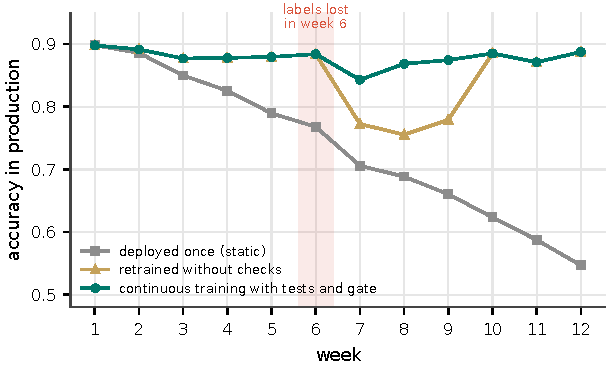
\includegraphics[width=0.78\textwidth]{ch05/continuous_training}
\caption{Accuracy in production of a static model, of weekly retraining without checks, and of continuous
training with a data test and a quality gate, under concept drift and a data incident in week 6.}
\label{fig:ct}
\end{figure}

The gate deserves a closer look. In this run it never rejects a candidate: every week with valid data
is promoted, once with a loss of 0.002 that lies within the tolerance, so the benefit shown comes from the
data test, not from the gate. The gate is a tolerance on a point estimate, not a statistical test of
non-inferiority. A production gate should fix in advance the loss it can accept and compare the two
models on the same examples with a paired measure of uncertainty (\cref{sec:stats}); failing to show that
the new model is better does not show that it is not worse.

Once a new version passes the gate, it can be released gradually \citep{huyen2022designing}: in \emph{shadow
mode}, it receives a copy of the production traffic but its predictions are not used; in a \emph{canary
release}, it serves a small fraction of the users, growing if everything goes well; in an \emph{A/B test},
the old and the new version serve random halves of the users, and the decision is made on business metrics
\citep{kohavi2020trustworthy}. Watching what happens after the release is the subject of Unit~6.

% ---------------------------------------------------------------------
\section{Case study: ModelOps for predictive maintenance}\label{sec:mannco}

\citet{dubovikov2019managing} describes a team that built predictive maintenance models for a manufacturing
company. The models had to be adapted and retrained constantly, and separately for each plant, and several
data scientists worked on them at the same time. The team assembled its infrastructure step by step:
\begin{itemize}
  \item \emph{collaboration and code management}: a GitLab server to share the code, and the GitFlow
        branching model so that everyone followed the same rules for features, releases and fixes;
  \item \emph{project structure}: a PyScaffold template with its data science extension, which gave every
        project the same layout for code, notebooks, data, models and documentation, and integrated well with
        Anaconda environments; repeated code was moved into the project's package, and stable code into its
        source and scripts directories, with a single entry point to train a new model version;
  \item \emph{data versioning}: DVC, with the company's internal file server as remote storage, and DVC
        pipelines to make every experiment reproducible;
  \item \emph{experiment tracking}: an MLflow server with a shared database, so that every team member could
        browse and compare the results of the models for the different plants;
  \item \emph{notebooks in pipelines}: the team liked to prototype in Jupyter notebooks, and used papermill to
        execute them from the command line as steps of the DVC pipelines;
  \item \emph{testing}: a suite of pytest tests, run by GitLab CI/CD on every commit;
  \item \emph{serving and delivery}: the customer wanted a simple API, so the models were served with MLflow,
        packaged with the code in Docker images built by GitLab CI/CD and pushed to a Docker registry.
\end{itemize}
The resulting process had seven steps: make changes to the code; run pre-commit checks of code quality and
style; run the tests in GitLab CI/CD; package the code and the trained models into a Docker image; push the
image to the registry; and, after a manual confirmation in the GitLab interface, run the update command on
the customer's server, which replaces the running container with the new version. Every tool in the list is
simple; what made the difference was combining them into a pipeline that runs without anyone having to
remember the steps.

% ---------------------------------------------------------------------
\section{Building your technology stack}\label{sec:stack}

There is no single right stack: the choice depends on the size of the team and of the project, on the
infrastructure of the organisation and its customers, and on the skills available. \Cref{tab:stack} lists
widely used open-source options for each need. Two principles help: start with the simplest tool that solves
a real problem (a CSV experiment log before a tracking server, a script before an orchestrator), and add
tools only when their benefit outweighs the cost of learning and maintaining them. A small, well-integrated
stack is better than a large collection of tools that nobody fully masters.

\begin{table}[htbp]
\centering\small
\caption{A toolbox for ModelOps.}\label{tab:stack}
\begin{tabularx}{\textwidth}{@{}>{\raggedright\arraybackslash}p{3.4cm}X@{}}
\toprule
Need & Tools\\
\midrule
Code collaboration & GitHub, GitLab, Bitbucket\\
Static code analysis & Flake8 (with extensions such as wemake), MyPy, pre-commit hooks\\
Project templates & PyScaffold (with its data science extension), Cookiecutter\\
Environments & venv/virtualenv, pyenv, pipenv, Poetry, Conda\\
Testing & pytest, Hypothesis\\
CI/CD servers & Jenkins, GitLab CI/CD, GitHub Actions, Travis CI, CircleCI\\
Data versioning & DVC, Git LFS\\
Pipelines & DVC pipelines, MLflow Projects\\
Experiment tracking & MLflow, Sacred, DVC\\
Model exchange & ONNX, PMML\\
Serving & Flask, FastAPI, MLflow models, TensorFlow Serving \citep{olston2017tensorflow}\\
Packaging and deployment & Docker, Kubernetes, Ansible\\
\bottomrule
\end{tabularx}
\end{table}

% ---------------------------------------------------------------------
\section{Summary}\label{sec:summary5}

\begin{itemize}
  \item The deployment option follows from the requirements of latency, hardware, network, privacy, cost and
        complexity. Streaming APIs answer each request when it arrives; batch jobs precompute predictions
        whose features are known in advance, much more efficiently; hybrid systems combine both at the price
        of complexity.
  \item Client-side deployment removes servers and keeps data on the device, but requires small models:
        quantisation, fewer features and distillation can shrink a model by orders of magnitude with little
        loss of accuracy.
  \item Federated learning trains a shared model from data that never leave the devices, and allows
        personalised models; updates must still be protected.
  \item Native serialisation ties production to the training environment and is unsafe with untrusted
        files. PMML is a declarative, auditable standard, popular in regulated industries; ONNX, a widely used open format, also covers deep learning and runs fast on servers, browsers and phones.
        Exported models must be checked against the originals.
  \item ModelOps adapts DevOps to data science, adding data versioning, experiment tracking and tests of data
        and models to version control, CI/CD, packaging and deployment.
  \item Continuous training pipelines retrain and redeploy models automatically; data tests and quality gates
        stop bad data and bad models from reaching production.
  \item Applications built on large language models are deployed as prompts, retrieval and guardrails around a
        model that runs behind an API or on the organisation's hardware. Prompts are code; the retriever can be
        measured with ranking metrics; outputs need tests; and prompt injection needs specific defences.
\end{itemize}

\section*{Bibliographic notes}
\addcontentsline{toc}{section}{Bibliographic notes}

\citet{ameisen2020building} covers the path from idea to deployed product, and \citet{huyen2022designing} the
design of production machine learning systems. \citet{dubovikov2019managing} describes ModelOps in the context
of managing data science teams, and \citet{kreuzberger2023mlops} survey MLOps. \citet{sculley2015hidden} and
\citet{paleyes2022challenges} are essential reading on what goes wrong in production. \citet{kairouz2021advances}
review federated learning, and \citet{humble2010continuous} is the classical reference on continuous delivery.

\section*{Exercises}
\addcontentsline{toc}{section}{Exercises}

\begin{enumerate}[label=\textbf{5.\arabic*},ref=5.\arabic*,leftmargin=*,itemsep=6pt]
  \item\label{exr5:choose} Choose a deployment option for each application and justify it: (a) the price of a
        taxi trip quoted when the user asks for it; (b) a daily ranking of the customers a call centre should
        contact; (c) word suggestions in a phone keyboard; (d) a model that reads medical images inside a
        hospital whose data may not leave the building.
  \item\label{exr5:little} A prediction service receives 200 requests per second. Each request occupies a worker for
        50 ms on average, and each server has four workers. How many requests are in the system on average,
        and what is the smallest number of servers whose idealised capacity exceeds the load?

  \item\label{exr5:batch} A model has a fixed cost of 8 ms per call plus 0.05 ms per example. Compute its
        throughput with batches of 1 and of 1000 examples.
  \item\label{exr5:quant} A neural network has 1.2 million parameters. How much memory do they need in 32-bit
        floating point, in 16-bit floating point and in 8-bit integers?
  \item\label{exr5:latency} Inference takes 120 ms on a phone and 15 ms on a server. The network round trip
        takes 80 ms, and the upload speed is 10 Mbit/s. Where should the model run if each request uploads a
        2 MB image? And if it uploads 20 kB of features?
  \item\label{exr5:fedavg} Three clients with 100, 300 and 600 examples return the values 0.2, 0.5 and 0.9 for a
        parameter. What value does federated averaging assign to it?
  \item\label{exr5:privacy} Why is sending model updates instead of data not enough to guarantee privacy? Name two
        techniques that improve it.
  \item\label{exr5:format} Choose a format to move each model, and justify it: (a) a credit scoring model
        that a regulator must audit and that runs in the bank's Java systems; (b) a gradient boosting model
        that must answer single requests in well under a millisecond; (c) an image classifier for Android
        phones and web browsers; (d) a model shared by two data scientists of the same team, who use the
        same environment.
  \item\label{exr5:pickle} Why should a pickle file from an unknown source never be loaded? Why is a PMML
        file safer?
  \item\label{exr5:dvc} Why is it a bad idea to commit a 2 GB CSV file that changes every day to Git? What does
        DVC store in Git instead?
  \item\label{exr5:tests} Classify as unit, integration or end-to-end test: (a) a function that parses dates
        returns the right value for ten formats; (b) the whole training pipeline runs on 1\% of the data and
        produces a model file; (c) the full pipeline is run on the complete data and the model reaches the
        expected accuracy. Propose an invariance test for a model that predicts house prices.
  \item\label{exr5:gate} A new model reaches an accuracy of 0.842 on 2000 validation examples and the production
        model 0.836 on the same examples. (a) Would a gate that promotes any positive difference promote it?
        (b) Is the improvement statistically supported if the new model is right and the old one wrong on 12
        examples and the opposite never happens? And if those counts are 112 and 100?

  \item\label{exr5:order} Put these steps of a continuous training pipeline in order: train a new model, run the
        unit tests, launch the new version, run data quality tests, package the model, fetch new data, test the
        quality of the model.
  \item\label{exr5:isolation} What does each of a virtual environment, a Conda environment and a Docker container
        isolate?
  \item\label{exr5:rag} A RAG assistant finds the right passage among the first three for 92\% of the questions of
        its test set, yet users complain that many of its answers are wrong. Give three possible causes and how you would
        check each of them.
\end{enumerate}

\section*{Solutions to selected exercises}
\addcontentsline{toc}{section}{Solutions to selected exercises}

\begin{description}[font=\bfseries,leftmargin=0pt,itemsep=5pt]
  \item[\ref{exr5:choose}] (a) Server-side streaming: the location and the available drivers exist only at request
        time. (b) Batch: the features are known in advance and nobody needs the ranking before the morning.
        (c) On device: low latency, offline use and private typing (possibly with federated learning).
        (d) On premises, on the hospital's own servers: the data cannot be sent to an external server.
  \item[\ref{exr5:little}] $L=200\cdot0.05=10$ requests in the system on average (Little's law counts waiting requests
        too). A worker serves about 20 requests per second and a server 80, so $200/80=2.5$: at least three
        servers, with an idealised utilisation of $200/240\approx0.83$. The margin for peaks, failures and tail
        latency is decided with a latency objective and a load test, not with Little's law.

  \item[\ref{exr5:batch}] One example per call: $1/8.05$ ms, about 124 predictions per second. Batches of 1000:
        $1000/(8+50)$ ms, about 17,200 per second.
  \item[\ref{exr5:quant}] 4.8 MB, 2.4 MB and 1.2 MB.
  \item[\ref{exr5:latency}] Uploading 2 MB at 10 Mbit/s takes 1.6 s, so the server needs about 1.7 s and the phone
        wins (120 ms). Uploading 20 kB takes 16 ms, so the server needs $80+16+15=111$ ms, slightly less than the
        phone; privacy, offline use and the cost of the servers may still favour the phone.
  \item[\ref{exr5:fedavg}] $(100\cdot0.2+300\cdot0.5+600\cdot0.9)/1000=0.71$.
  \item[\ref{exr5:privacy}] Updates are computed from the data, and an attacker can reconstruct training examples
        from them. Secure aggregation, so that the server sees only the sum of many updates, and differential
        privacy, which adds calibrated noise.
  \item[\ref{exr5:format}] (a) PMML: declarative, readable and auditable, and scored by Java engines. (b) ONNX with
        ONNX Runtime, which avoids the overhead of the Python pipeline at every call (\cref{lst:onnx}); whether it
        meets the budget must be checked with a representative benchmark on the target hardware. (c) ONNX, run
        by ONNX Runtime on Android and by ONNX Runtime Web in the browser, after checking that both support its
        operators; or a LiteRT model for Android plus a separate export for the browser, each with its runtime.
        (d) joblib or pickle, with pinned versions, or an MLflow model.

  \item[\ref{exr5:pickle}] Unpickling can call arbitrary functions chosen by whoever wrote the file, so it can
        execute any code on the machine. A PMML file only describes the model: an engine that implements the
        standard computes the predictions, and no code from the author of the file is run.
  \item[\ref{exr5:dvc}] Git records snapshots, and every daily version of a 2 GB file adds another large object
        (delta compression helps little with such files), so cloning and every operation slow down. DVC keeps a
        small reference to each version in Git and the data elsewhere, and its \texttt{dvc.lock} records which
        data produced which model.

  \item[\ref{exr5:tests}] (a) Unit, (b) integration, (c) end-to-end. Invariance: the predicted price must not change
        when only the identifier of the listing changes, with every feature of the property, including its
        location, held fixed; the name of the street can encode the location, so changing it is not an
        irrelevant transformation.
  \item[\ref{exr5:gate}] (a) Yes: the difference is 0.006, twelve more correct predictions. (b) The answer depends on
        the paired disagreements, not on the two accuracies. With 12 and 0, the exact McNemar test gives
        $p\approx0.0005$: evidence of a difference. With 112 and 100, $p\approx0.45$: no evidence. The standard error of
        one accuracy (about 0.008) is not that of the difference. And not rejecting equality does not show that
        the models are equivalent: a non-inferiority decision needs a margin fixed in advance.

  \item[\ref{exr5:order}] Run the unit tests; fetch new data; run data quality tests; train a new model; test its
        quality; package the model; launch the new version.
  \item[\ref{exr5:isolation}] A virtual environment isolates the Python packages; a Conda environment also isolates
        the Python version and non-Python libraries; a container isolates the whole user space of the operating
        system, including system libraries and configuration. A container shares the kernel of the host.

  \item[\ref{exr5:rag}] (1) The right passage is often not the first one (in \cref{lst:rag}, only 67\% at rank 1) and the
        prompt includes too few passages: measure recall at the number of passages actually used. (2) The test set does not
        look like real questions: sample real questions from the logs and evaluate on them. (3) The model does not use the
        passages, or contradicts them: measure the groundedness of the answers on a sample, by people or with a validated
        judge. Outdated documents in the index are a fourth candidate.
\end{description}

